\chapter{基于深度学习方法的低分辨率环境下微表情识别}\label{chap:owner2}

我们考虑在不受控制的环境中对动作的全自动识别。大多数现有的工作依赖领域知识从输入构建复杂的手工特性。此外,通常假定环境是受控的。卷积神经网络(Convolutional Neural Networks,CNN)是一种深度模型,它可以直接作用于原始输入,从而实现特征构造过程的自动化。然而,这些模型目前仅限于处理2D输入。在本文中,我们开发了一种新的三维CNN动作识别模型。该模型通过三维卷积从空间和时间两个维度提取特征,从而获取多个相邻帧中编码的运动信息。所建立的模型从输入帧中生成多个通道的信息,并结合所有通道的信息得到最终的特征表示。我们将开发的模型应用到现实环境中的人类行为识别中,在不依赖于手工制作的特性的情况下取得了优异的性能。

微表情是检测谎言的重要线索之一。它最突出的特点是运动时间短、强度低。因此,高时空分辨率的视频片段比静止图像更需要提供足够的细节。另一方面,由于微表达数据的采集和编码困难,样本量较小。在本文中,我们仅使用560个微表情视频片段来评价所提出的转移长期卷积神经网络(Transfer Long-term Convolutional Neural Network,TLCNN)。TLCNN利用深度CNN从微表情视频片段的每一帧中提取特征,然后将其输入到长短期记忆网络(Long Short-Term Memory,LSTM)中,LSTM学习微表情的时序信息。由于微表情数据的样本容量较小,TLCNN采用了两个迁移学习的步骤:(1)从表情数据进行迁移,(2)从单帧微表情视频片段进行迁移,可视为“大数据”。对采集自三个自发性数据库的560个微表情视频片段进行评价。结果表明,所提出的TLCNN算法优于现有的一些算法。

近年来,随着计算机硬件特别是图形处理器(Graphics Processing Unit,GPU)的飞速发展,深度学习在人脸识别、验证等领域得到了广泛的应用,表现出了优异的性能。这些深度学习方法使用多个处理层来发现非常大的数据集中的模式和结构。每一层从后续层构建的数据中学习一个概念;层次越高,所学的概念就越抽象。深度学习不依赖于先验数据处理,自动提取特征。这些优势和深度学习的良好表现都归功于大数据。然而,微表情视频片段的数量通常很少。在样本容量较小的数据上进行深度学习可能不会取得良好的效果。针对这一问题,我们利用转移学习对深度卷积神经网络进行预处理,提出了用于微表情识别的TLCNN网络。在TLCNN中,迁移学习有两个步骤:(1)从表情数据进行迁移,(2)从单个微表达视频片段帧进行迁移,这可以看作是大数据。为了充分利用微表情视频中的时间信息,TLCNN还利用LSTM从每帧图像的中层图像表示中提取微表情视频的时间特征。

\begin{figure}[!htb]
\centering
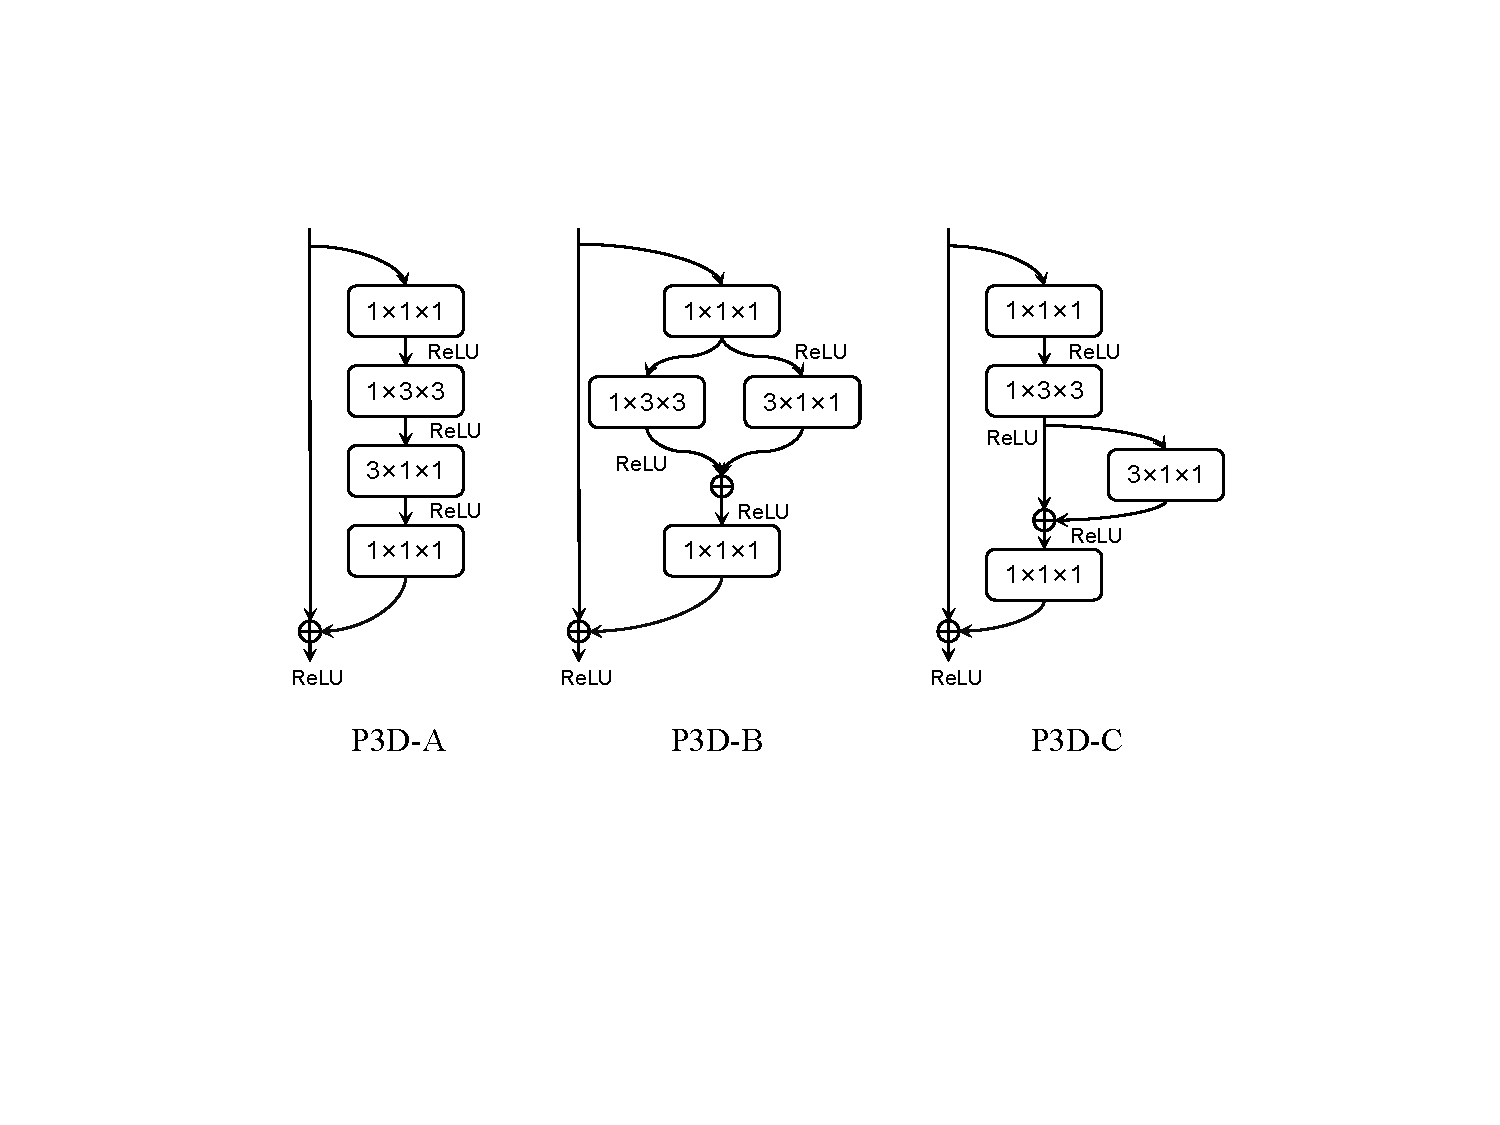
\includegraphics[width=1\textwidth]{P3D0}
\caption{基于深度学习方法的低分辨率环境下微表情识别网络框架}
\label{fig20}
\end{figure}

\section{数据集预处理}

提取深度特征需要庞大的数据量支持,然而因为微表情的特殊性导致目前发表的数据集很少,所以对现有数据进行增强处理很有必要。数据增强(Data Augmentation)一般是指对图片进行随机的旋转、翻转、裁剪、随机设置图片的亮度和对比度以及对数据进行标准化(数据的均值为0,方差为1)。通过对数据增强的操作,可以让我们原本匮乏的数据变得稍微丰富。将原来的一张图片变为多张图片,这样扩大了样本容量,对于提高模型的准确率和提升模型的泛化能力非常有帮助。在本文中根据微表情数据的特殊性选择了其中的直方图均衡化、图像亮度变化和水平翻转三种方式,同时将现有的SMIC-HS和CASME II两个数据集做了融合,使得最终达到4233个片段,让模型的泛化能力进一步得到提升。

\subsection{数据集融合}

将SMIC-HS和CASME II两个数据集交叉融合,相似类归为一类。由原来的16个subject(SMIC-HS数据集)和26个subject(CASME II数据集)组合为现在的42个subject,如表~\ref{tab8}所示。

\begin{table}[!htbp]
\renewcommand\arraystretch{1.5}
\centering
\caption{融合后数据集情况}
\label{tab8}
\scalebox{0.85}{
\begin{tabular}{c|c|c|c}
\hline
表情类 & 片段数 & \multicolumn{2}{c}{数据来源} \\ \hline
POSITIVE & 83 & 51(SMIC-HS,Positive) & 32(CASME II,Happy) \\
NEGAYIVE & 134 & 70(SMIC-HS,Positive) & 64(CASME II,Disgust) \\
SURPRISE & 68 & 43(SMIC-HS,Surprise) & 25(CASME II,Surprise) \\
OTHERS & 126 & 99(CASME II,Others) & 27(CASME II,Repression) \\ \hline
\end{tabular}}
\end{table}

论文\citepns{Li2013A}将第一版的SMIC数据集由原来的五类标签合并为最终的三类,文中提到将第一版本的快乐分类(Happy)改为新的积极分类(Positive),新的消极分类(Negative)则是由第一版的悲伤(Sadness)、恐惧(Fear)和厌恶(Disgust)三个分类组合而成。按照上述这种合并方式我们将CASME II中的快乐分类与SMIC-HS中的积极分类合并组成新的积极分类,将CASME II中的厌恶分类与SMIC-HS中的消极分类合并组成新的消极分类,将两种数据集的惊讶分类合并组成新的惊讶分类,将CASME II的压抑分类和其他分类合并组成新的其他分类。

\subsection{数据增强}

直方图均衡化

直方图均衡化(Histogram Equalization) 又称直方图平坦化,实质上是对图像进行非线性拉伸,重新分配图像象元值,使一定灰度范围内象元值的数量大致相等。这样,原来直方图中间的峰顶部分对比度得到增强,而两侧的谷底部分对比度降低,输出图像的直方图是一个较平的分段直方图:如果输出数据分段值较小的话,会产生粗略分类的视觉效果。

直方图是表示数字图像中每一灰度出现频率的统计关系。直方图能给出图像灰度范围、每个灰度的频度和灰度的分布、整幅图像的平均明暗和对比度等概貌性描述。灰度直方图是灰度级的函数, 反映的是图像中具有该灰度级像素的个数, 其横坐标是灰度级$r$, 纵坐标是该灰度级出现的频率(即像素的个数) $p_{r}(r)$, 整个坐标系描述的是图像灰度级的分布情况, 由此可以看出图像的灰度分布特性, 即若大部分像素集中在低灰度区域, 图像呈现暗的特性; 若像素集中在高灰度区域, 图像呈现亮的特性。

图~\ref{fig20}所示就是直方图均衡化, 即将随机分布的图像直方图修改成均匀分布的直方图。基本思想是对原始图像的像素灰度做某种映射变换, 使变换后图像灰度的概率密度呈均匀分布。这就意味着图像灰度的动态范围得到了增加, 提高了图像的对比度。

通过这种技术可以清晰地在直方图上看到图像亮度的分布情况, 并可按照需要对图像亮度调整。另外,这种方法是可逆的, 如果已知均衡化函数, 就可以恢复原始直方图。

设变量$r$代表图像中像素灰度级。对灰度级进行归一化处理, 则$0\leqslant r\leqslant 1$ , 其中$r=0$表示黑,$r=1$表示白。对于一幅给定的图像来说, 每个像素值在[0,1]的灰度级是随机的。用概率密度函数$p_{r}(r)$ 来表示图像灰度级的分布。

为了有利于数字图像处理, 引入离散形式。在离散形式下, 用$r_{k}$ 代表离散灰度级, 用$p_{r}(r_{k})$ 代表$p_{r}(r)$ , 并且下式成立:$p_{r}(r_{k})=n_{k}/n$,其中,$0\leqslant r_{k}\leqslant 1$,$k=0,1,2,\cdots ,L-1$ 。式中$n_{k}$为图像中出现$r_{k}$这种灰度的像素数, $n$是图像中的像素总数, 而$n_{k}/n$就是概率论中的频数。图像进行直方图均衡化的函数表达式为:
\begin{equation}
 \label{eq6}
 \begin{split}
   S_{i}=T(r_{i})=\sum_{i=0}^{k-1}\frac{n_{i}}{n}
 \end{split}
\end{equation}
式中, $k$为灰度级数。相应的反变换为:
\begin{equation}
 \label{eq7}
 \begin{split}
   r_{i}=T^{-1}(S_{i})
 \end{split}
\end{equation}

\section{特征提取及识别}

P3D效果比C3D好太多

其他还有I3D、ResNet和P3D

T3D效果好点,但提升不大,且不好训练

I3D则要结合传统特征

\subsection{伪3D块}

受最近残差网络(ResNet)在众多具有挑战性的图像识别任务中取得成功的启发,我们开发了一个名为伪3D(P3D)块的构建模块族,以取代ResNet中的2D残差单元,在视频的ResNet-like架构中实现时空编码。接下来,我们将回顾ResNet中剩余单元的基本设计,然后介绍如何设计P3D块。最后阐述了每个P3D块上的瓶颈构建体系结构。

残差单位

ResNet由许多残余单元组成,每个残余单元通常由:
\begin{equation}
\label{eq8}
   \textbf{x}_{t+1}=\textbf{h}(\textbf{x}_{t})+\textbf{F}(\textbf{x}_{t})
\end{equation}
组成,其中$\textbf{x}_{t}$和$\textbf{x}_{t+1}$表示第$t$个残差单元的输入和输出,$\textbf{h}(\textbf{x}_{t})=\textbf{x}_{t}$为恒等映射,$\textbf{F}$为非线性残差函数。如图~\ref{fig9}所示。因此,式~\ref{eq8}可以改写为:
\begin{equation}
\label{eq9}
   (\textbf{I}+\textbf{F})\cdot \textbf{x}_{t}=\textbf{x}_{t}+\textbf{F}\cdot \textbf{x}_{t}:=\textbf{x}_{t}+\textbf{F}(\textbf{x}_{t})=\textbf{x}_{t+1}
\end{equation}
其中$\textbf{F}\cdot \textbf{x}_{t}$表示在$\textbf{x}_{t}$上执行残差函数$\textbf{F}$的结果。ResNet的主要思想是通过一个快捷的连接来学习参考单元输入$\textbf{x}_{t}$的可加性残差函数$\textbf{F}$,而不是直接学习未引用的非线性函数。

P3D块设计

为了将ResNet中的每个2D残差单元更改成用于编码时空视频信息的3D结构,我们按照3.1节中介绍的伪3D原理对ResNet中的基本残差单元进行了修改,并设计了几个伪3D块。由于涉及两个设计问题,所以修改并不简单。第一个问题是空间维度($\textbf{S}$)上的二维滤波器模块和时间域($\textbf{T}$)上的一维滤波器模块是否应该直接或间接地相互影响。两种滤波器之间的直接影响是将空间二维滤波器的输出作为时间一维滤波器的输入(即,以级联的方式连接)。两个滤波器之间的间接影响使连接分离,使每一种滤波器在网络的不同路径上(即,以并联的方式连接)。第二个问题是这两种滤波器是否都应该直接影响最终的输出。因此,在此上下文中,直接影响表示每种滤波器的输出都应该直接连接到最终输出。

基于这两个设计问题,我们推导出如图2所示的三个不同的P3D块,分别命名为P3D-A、P3D-B和P3D-C。关于它们的架构的详细比较如下:

(1)P3D-A:第一种设计考虑层加结构,使时间一维滤波器($\textbf{T}$)以级联方式跟随空间二维滤波器($\textbf{S}$)。因此,两种滤波器在同一路径上可以直接相互影响,时间一维滤波器直接连接到最终输出:
\begin{equation}
\label{eq10}
   (\textbf{I}+\textbf{T}\cdot\textbf{S})\cdot \textbf{x}_{t}:=\textbf{x}_{t}+\textbf{T}(\textbf{S}(\textbf{x}_{t}))=\textbf{x}_{t+1}
\end{equation}

(2)P3D-B:第二种设计与第一种设计相似,考虑了两种滤波器之间的间接影响,两种滤波器以并行的方式分布在不同的路径上。虽然$\textbf{S}$和$\textbf{T}$之间没有直接的影响,但是它们都直接累加到最终的输出中,可以表示为:
\begin{equation}
\label{eq11}
   (\textbf{I}+\textbf{S}+\textbf{T})\cdot \textbf{x}_{t}:=\textbf{x}_{t}+\textbf{S}(\textbf{x}_{t})+\textbf{T}(\textbf{x}_{t})=\textbf{x}_{t+1}
\end{equation}

(3)P3D-C:最后一个设计是在P3D-A和P3D-B之间寻求折中,即同时建立了$\textbf{S}$、$\textbf{T}$和最终输出之间的直接影响。具体来说,为了基于级联P3D-A结构实现$\textbf{S}$与最终输出的直接连接,我们建立了$\textbf{S}$到最终输出的连接,使输出$\textbf{x}_{t+1}$为:
\begin{equation}
\label{eq12}
   (\textbf{I}+\textbf{S}+\textbf{T}\cdot \textbf{S})\cdot \textbf{x}_{t}:=\textbf{x}_{t}+\textbf{S}(\textbf{x}_{t})+\textbf{T}(\textbf{S}(\textbf{x}_{t}))=\textbf{x}_{t+1}
\end{equation}

瓶颈(Bottleneck)结构

在确定二维残差单元的结构时,对二维基本块进行瓶颈设计,以降低计算复杂度。特别的,如图3所示(a),残差单位采用$1\times1$、$3\times3$和$1\times1$三层叠加的卷积网络,而不是一个单一的二维滤波器($3\times3$卷积),其中第一个和最后一个$1\times1$卷积层的作用分别是减少和恢复输入样本的维度。这种瓶颈设计使得中间的$3\times3$卷积层成为瓶颈,这种瓶颈结构具有更小的输入和输出维度。因此,我们按照这种完美的结构实现提出的P3D设计:由一个空间二维滤波器($1\times3\times3$卷积)和一个时间一维滤波器($3\times1\times1$卷积)组合成主要部分,同时将两个$1\times1\times1$卷积添加在路径的两端,负责对维度的降低和恢复。从而,该瓶颈结构减少了空间二维滤波器和时间一维滤波器的输入、输出维度。图3(b)-3(d)展示了这三个P3D块上详细的瓶颈构建体系结构。

\subsection{P3D ResNet}

为了验证三个P3D模块的优点,我们首先开发了三个P3D ResNet变体,即, P3D-A ResNet、P3D-B ResNet和P3D-C ResNet,分别用一种P3D块替换50层ResNet (ResNet-50)中的所有残余单元。比较了基本ResNet-50和三种P3D ResNet变体的性能和时间效率。然后,从结构多样性的角度,将三个P3D块混合在一起,提出了一个完整的P3D ResNet版本。

混合不同的P3D块。最近在深度网络设计中追求结构多样性的成功案例进一步激发了我们的设计灵感,促使我们设计了一个完整的P3D ResNet版本,通过在结构中混合不同的P3D块来增强结构多样性,如图4所示。特别地,我们按照P3D-A、P3D-B和P3D-C这样顺序的P3D链替换剩余的单元。表1详细说明了完整P3D ResNet的性能和速度。通过进一步追求结构多样性,P3D ResNet相对于P3D-A ResNet、P3D-B ResNet和P3D-C ResNet的准确率分别提高了0.5\%、1.4\%和1.2\%,说明随着深度的增加,结构多样性的增强可以提高神经网络的能力。

在视频分类或理解领域,容易从图像领域的2D卷积联想到用3D卷积来做,虽然用3D卷积进行特征提取可以同时考虑到空间和时间维度的特征,但是计算成本和模型存储都太大,因此这篇文章针对视频领域中采用的3D卷积进行改造,提出Pseudo-3D Residual Net(P3D ResNet),思想有点像当年的Inception v3中用$1\times3$和$3\times1$的卷积叠加代替原来的$3\times3$卷积,这篇文章是用$1\times3\times3$卷积和$3\times1\times1$卷积代替$3\times3\times3$卷积(前者用来获取空间维度的特征,实际上和2D的卷积没什么差别;后者用来获取时间维度的特征,因为倒数第三维是帧的数量),毕竟这样做可以大大减少计算量,而如果采用3D卷积来做的话,速度和存储正是瓶颈,这也使得像C3D算法的网络深度只有11层,参看图1。该文章的网络结构可以直接在3D的ResNet网络上修改得到。顺便提一下,除了采用3D卷积来提取时间维度上的特征外,还可以采用LSTM来提取,这也是当前视频研究的一个方向。

\begin{figure}[!htbp]
\centering
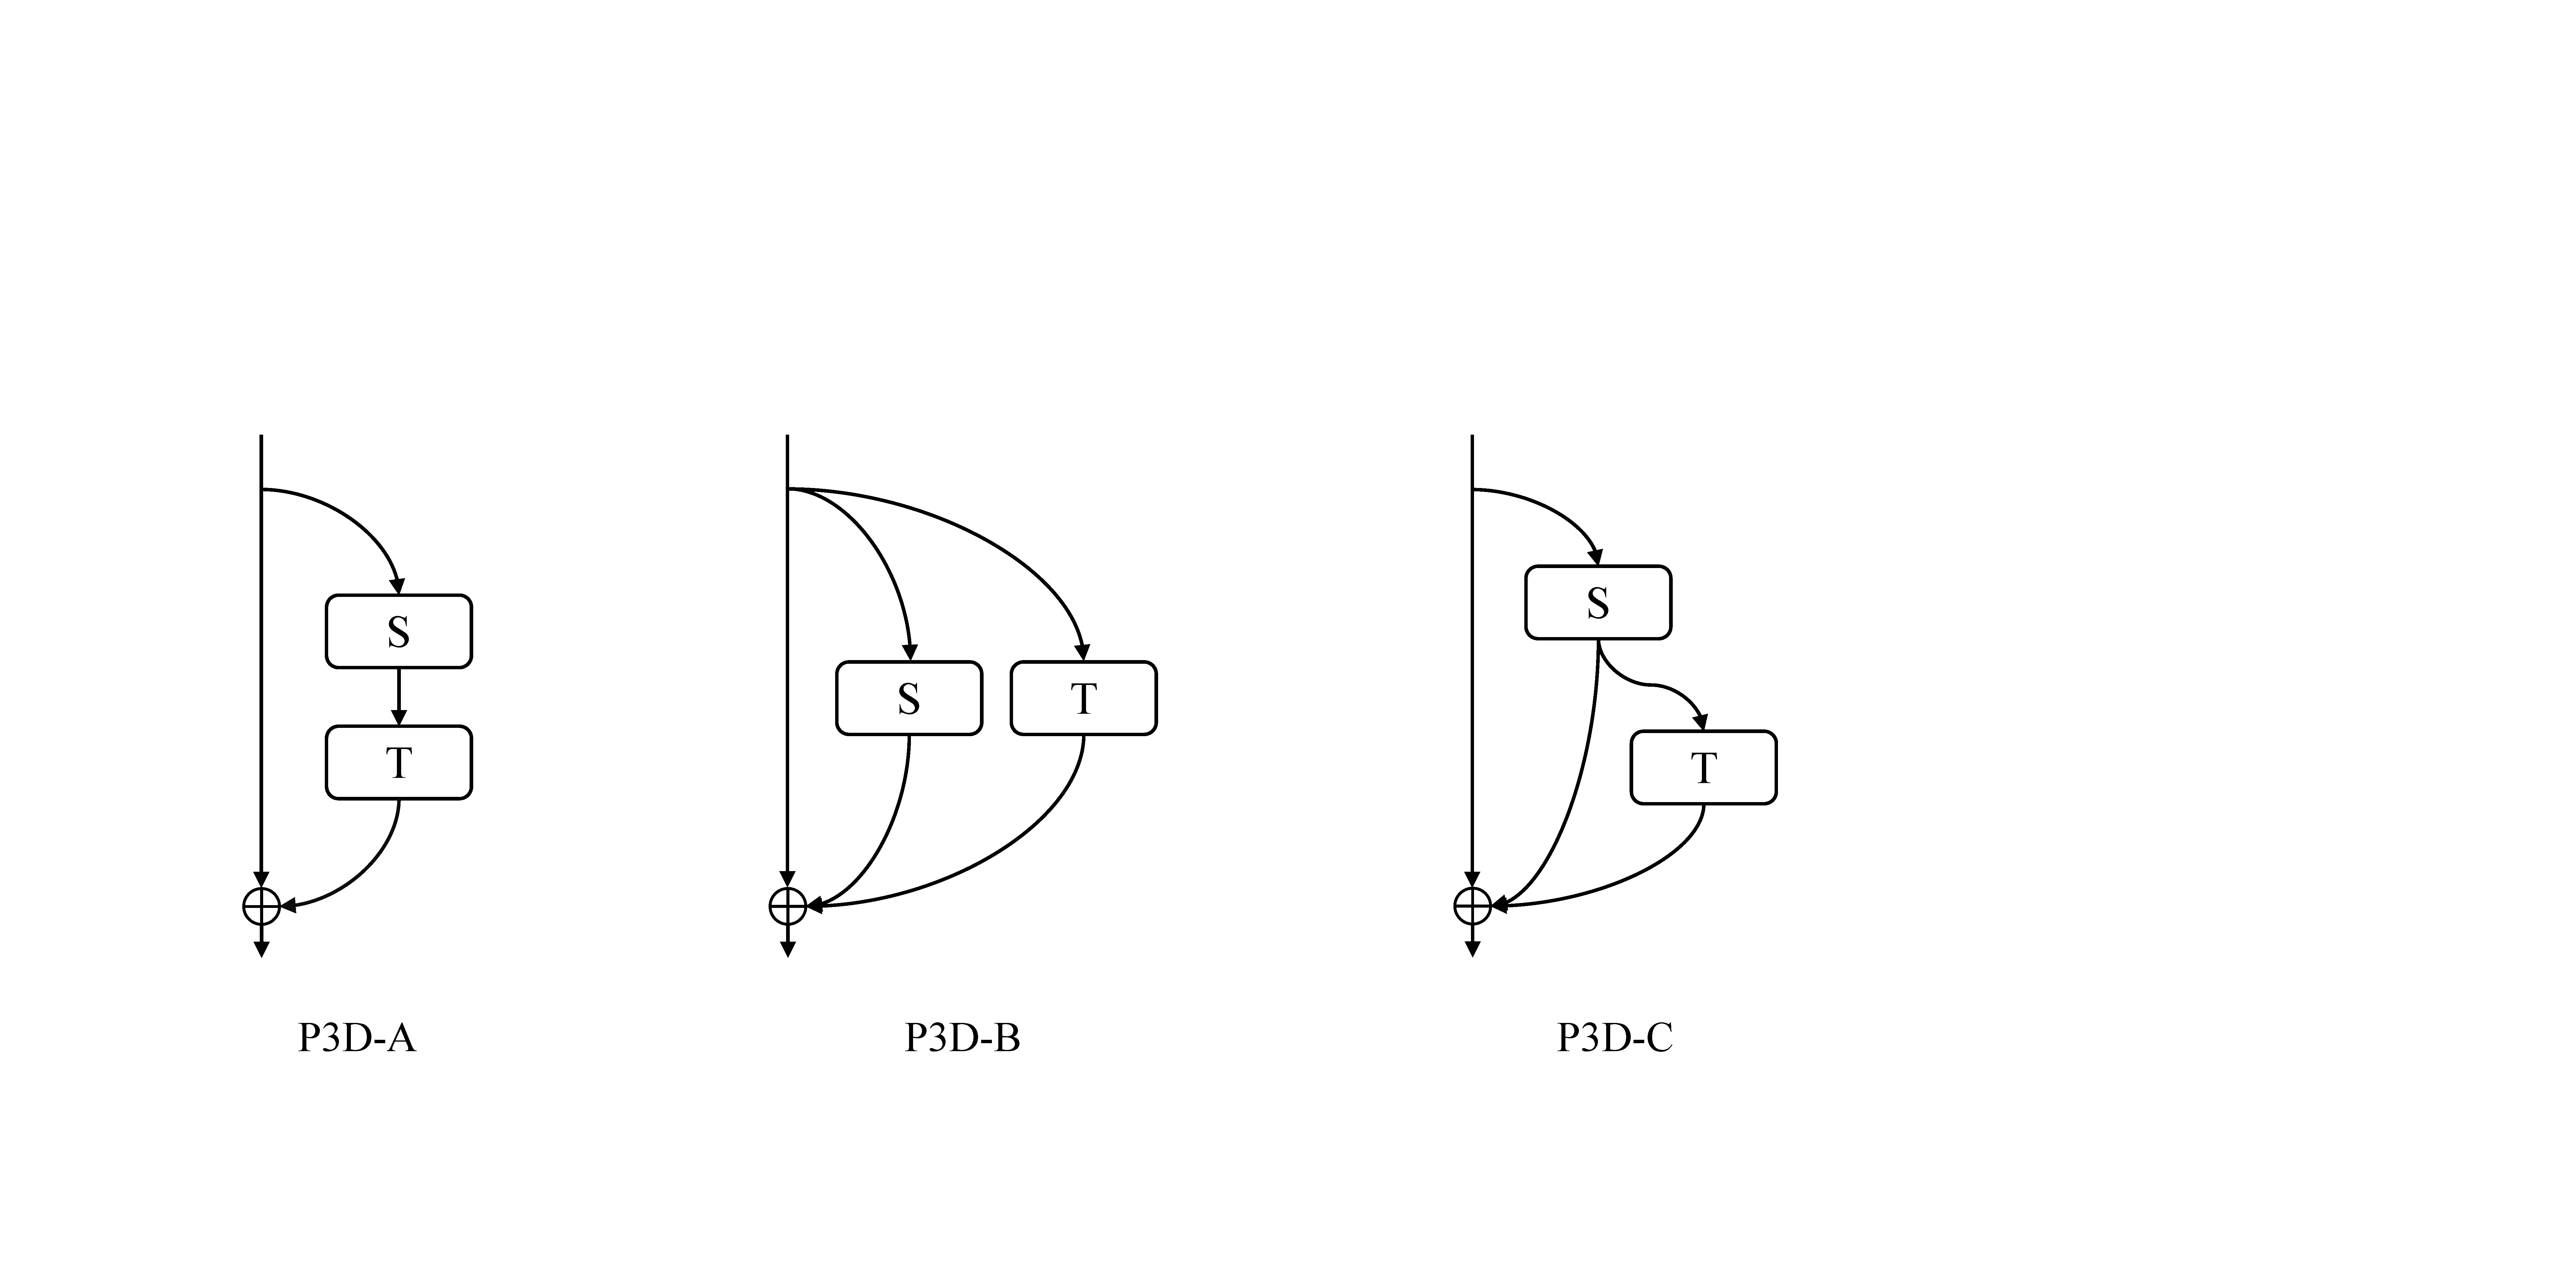
\includegraphics[width=0.80\textwidth]{P3D1}
\caption{三种P3D块设计}
\label{fig22}
\end{figure}

图1是几个模型在层数、模型大小和在Sports-1M数据集上的视频分类效果对比,其中的P3D ResNet是在ResNet 152基础上修改得到的,深度之所以不是152,是因为改造后的每个残差结构不是原来ResNet系列的3个卷积层,而是3或4个卷积层,详细可以看图3,所以最后网络深度是199层。官方GitHub代码中的网络就是199层的。ResNet 152是直接在Sports-1M数据集上Fine-Tune得到的。可以看出199层的P3D ResNet虽然在模型大小上比ResNet-152(此处ResNet-152是在sports-1M数据集上fine tune得到的)大一些,但是准确率提升比较明显,与C3D(此处C3D是直接在sports-1M数据集上从头开始训练得到的)的对比在效果和模型大小上都有较大改进,除此之外,速度的提升也是亮点,后面有详细的速度对比。

\begin{figure}[!htbp]
\centering
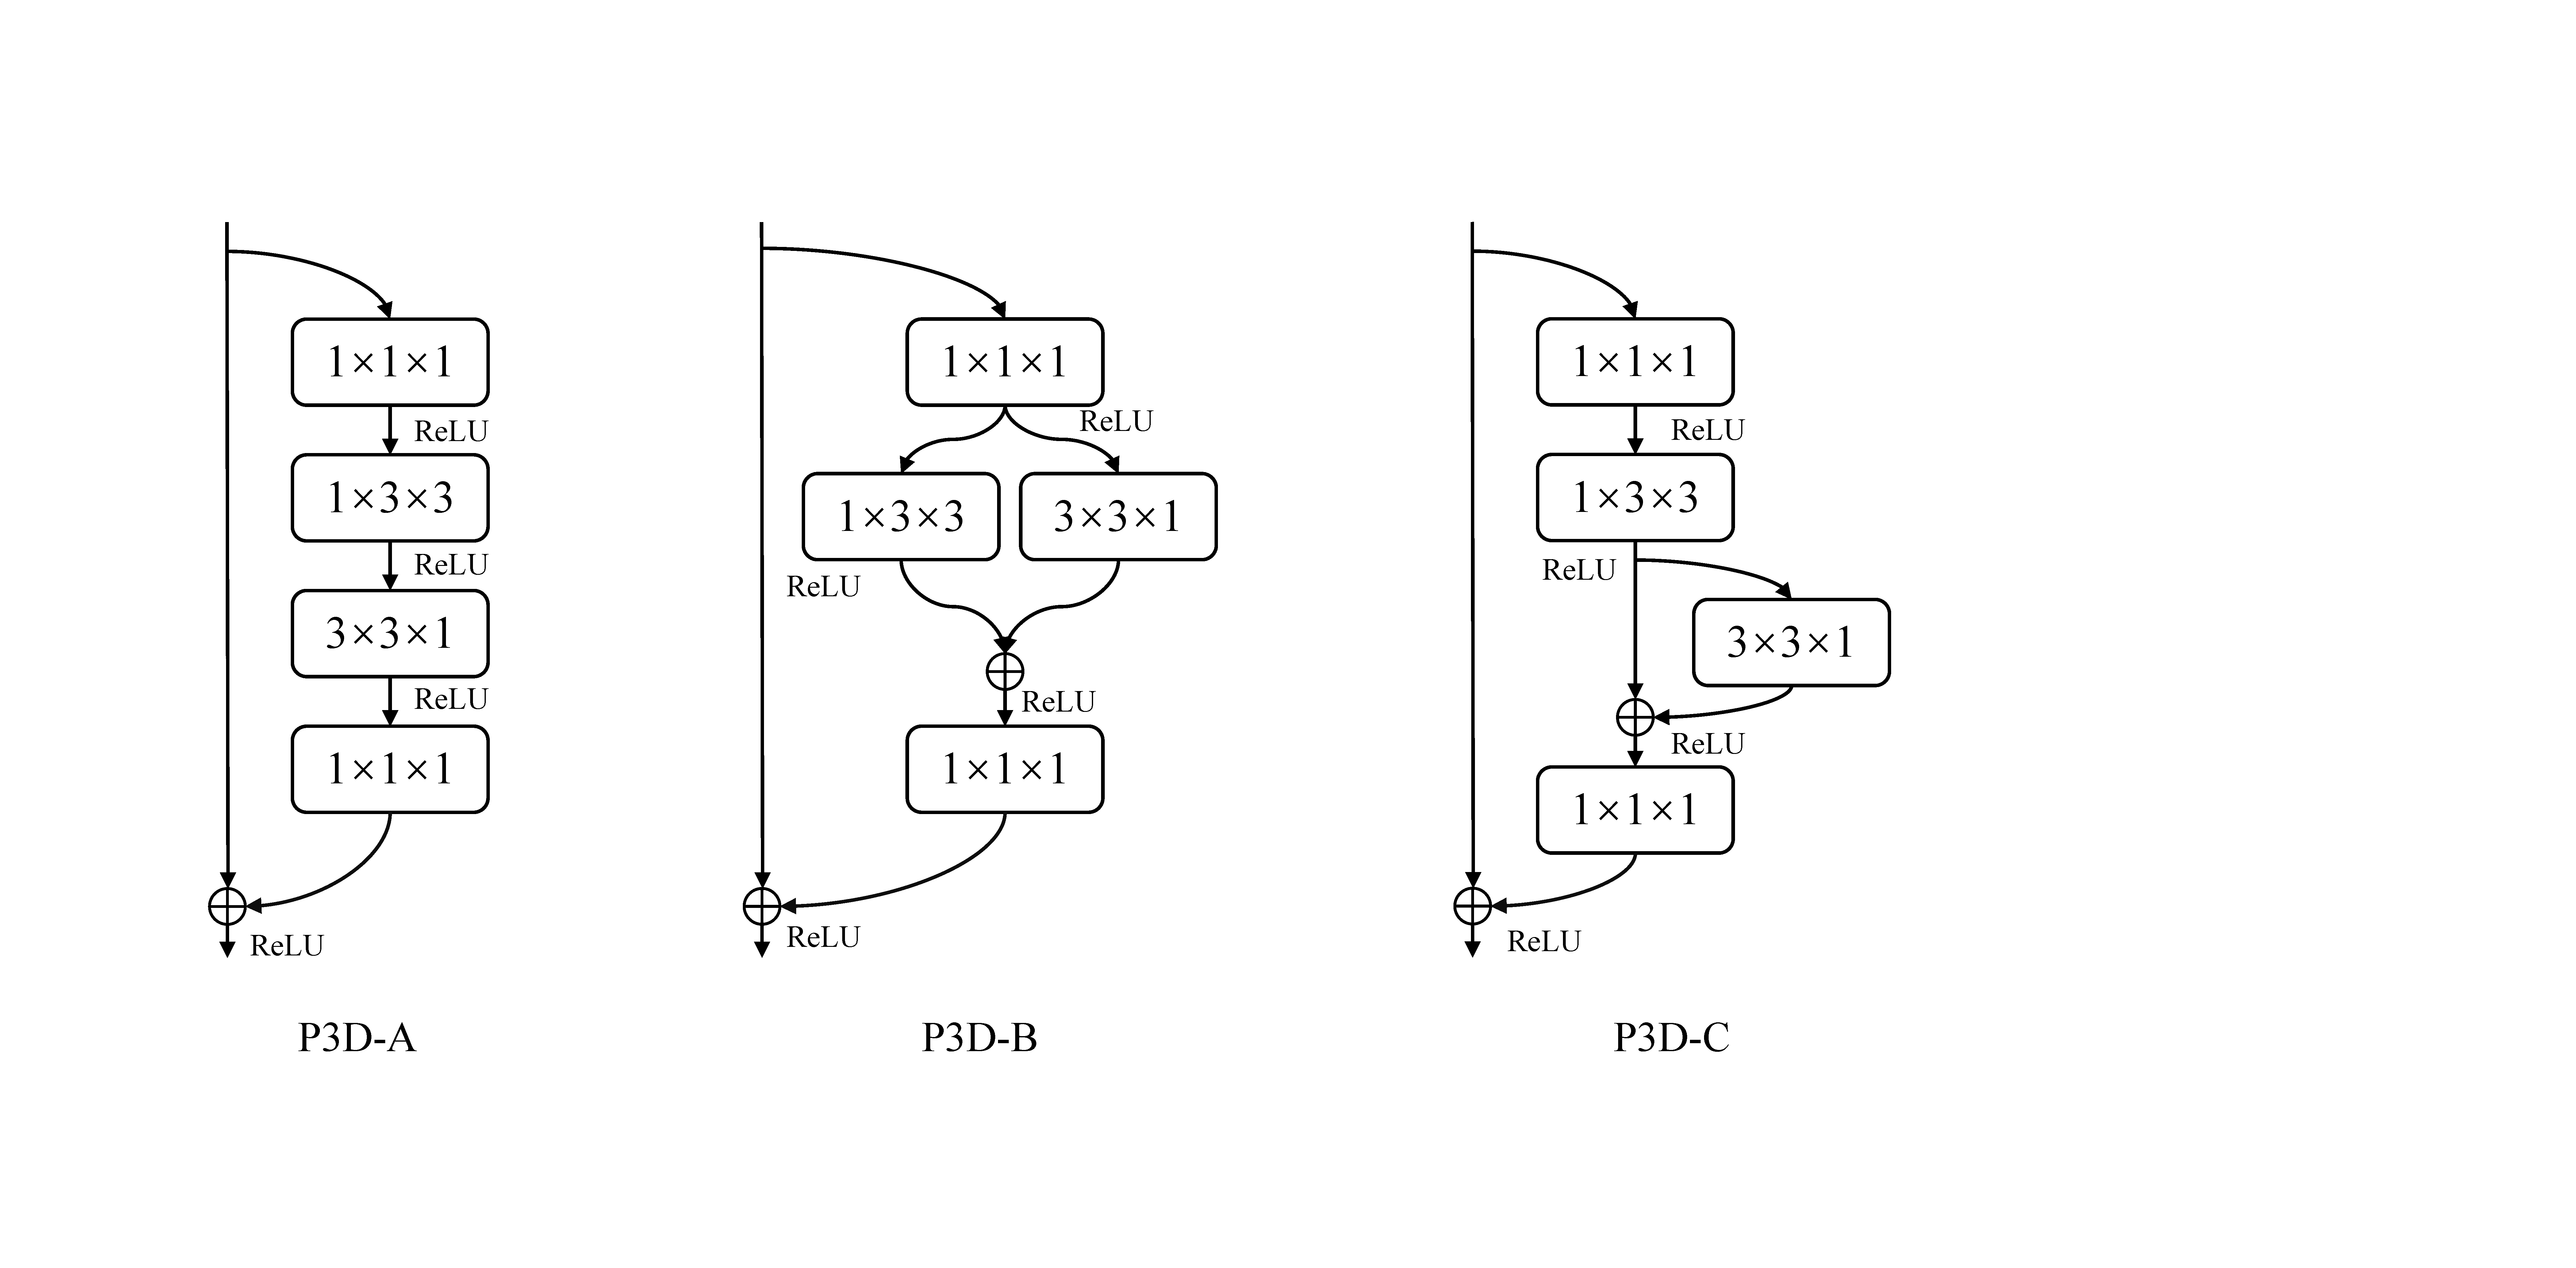
\includegraphics[width=0.80\textwidth]{P3D2}
\caption{三种P3D瓶颈块结构设计}
\label{fig23}
\end{figure}

\begin{figure}[!htbp]
\centering
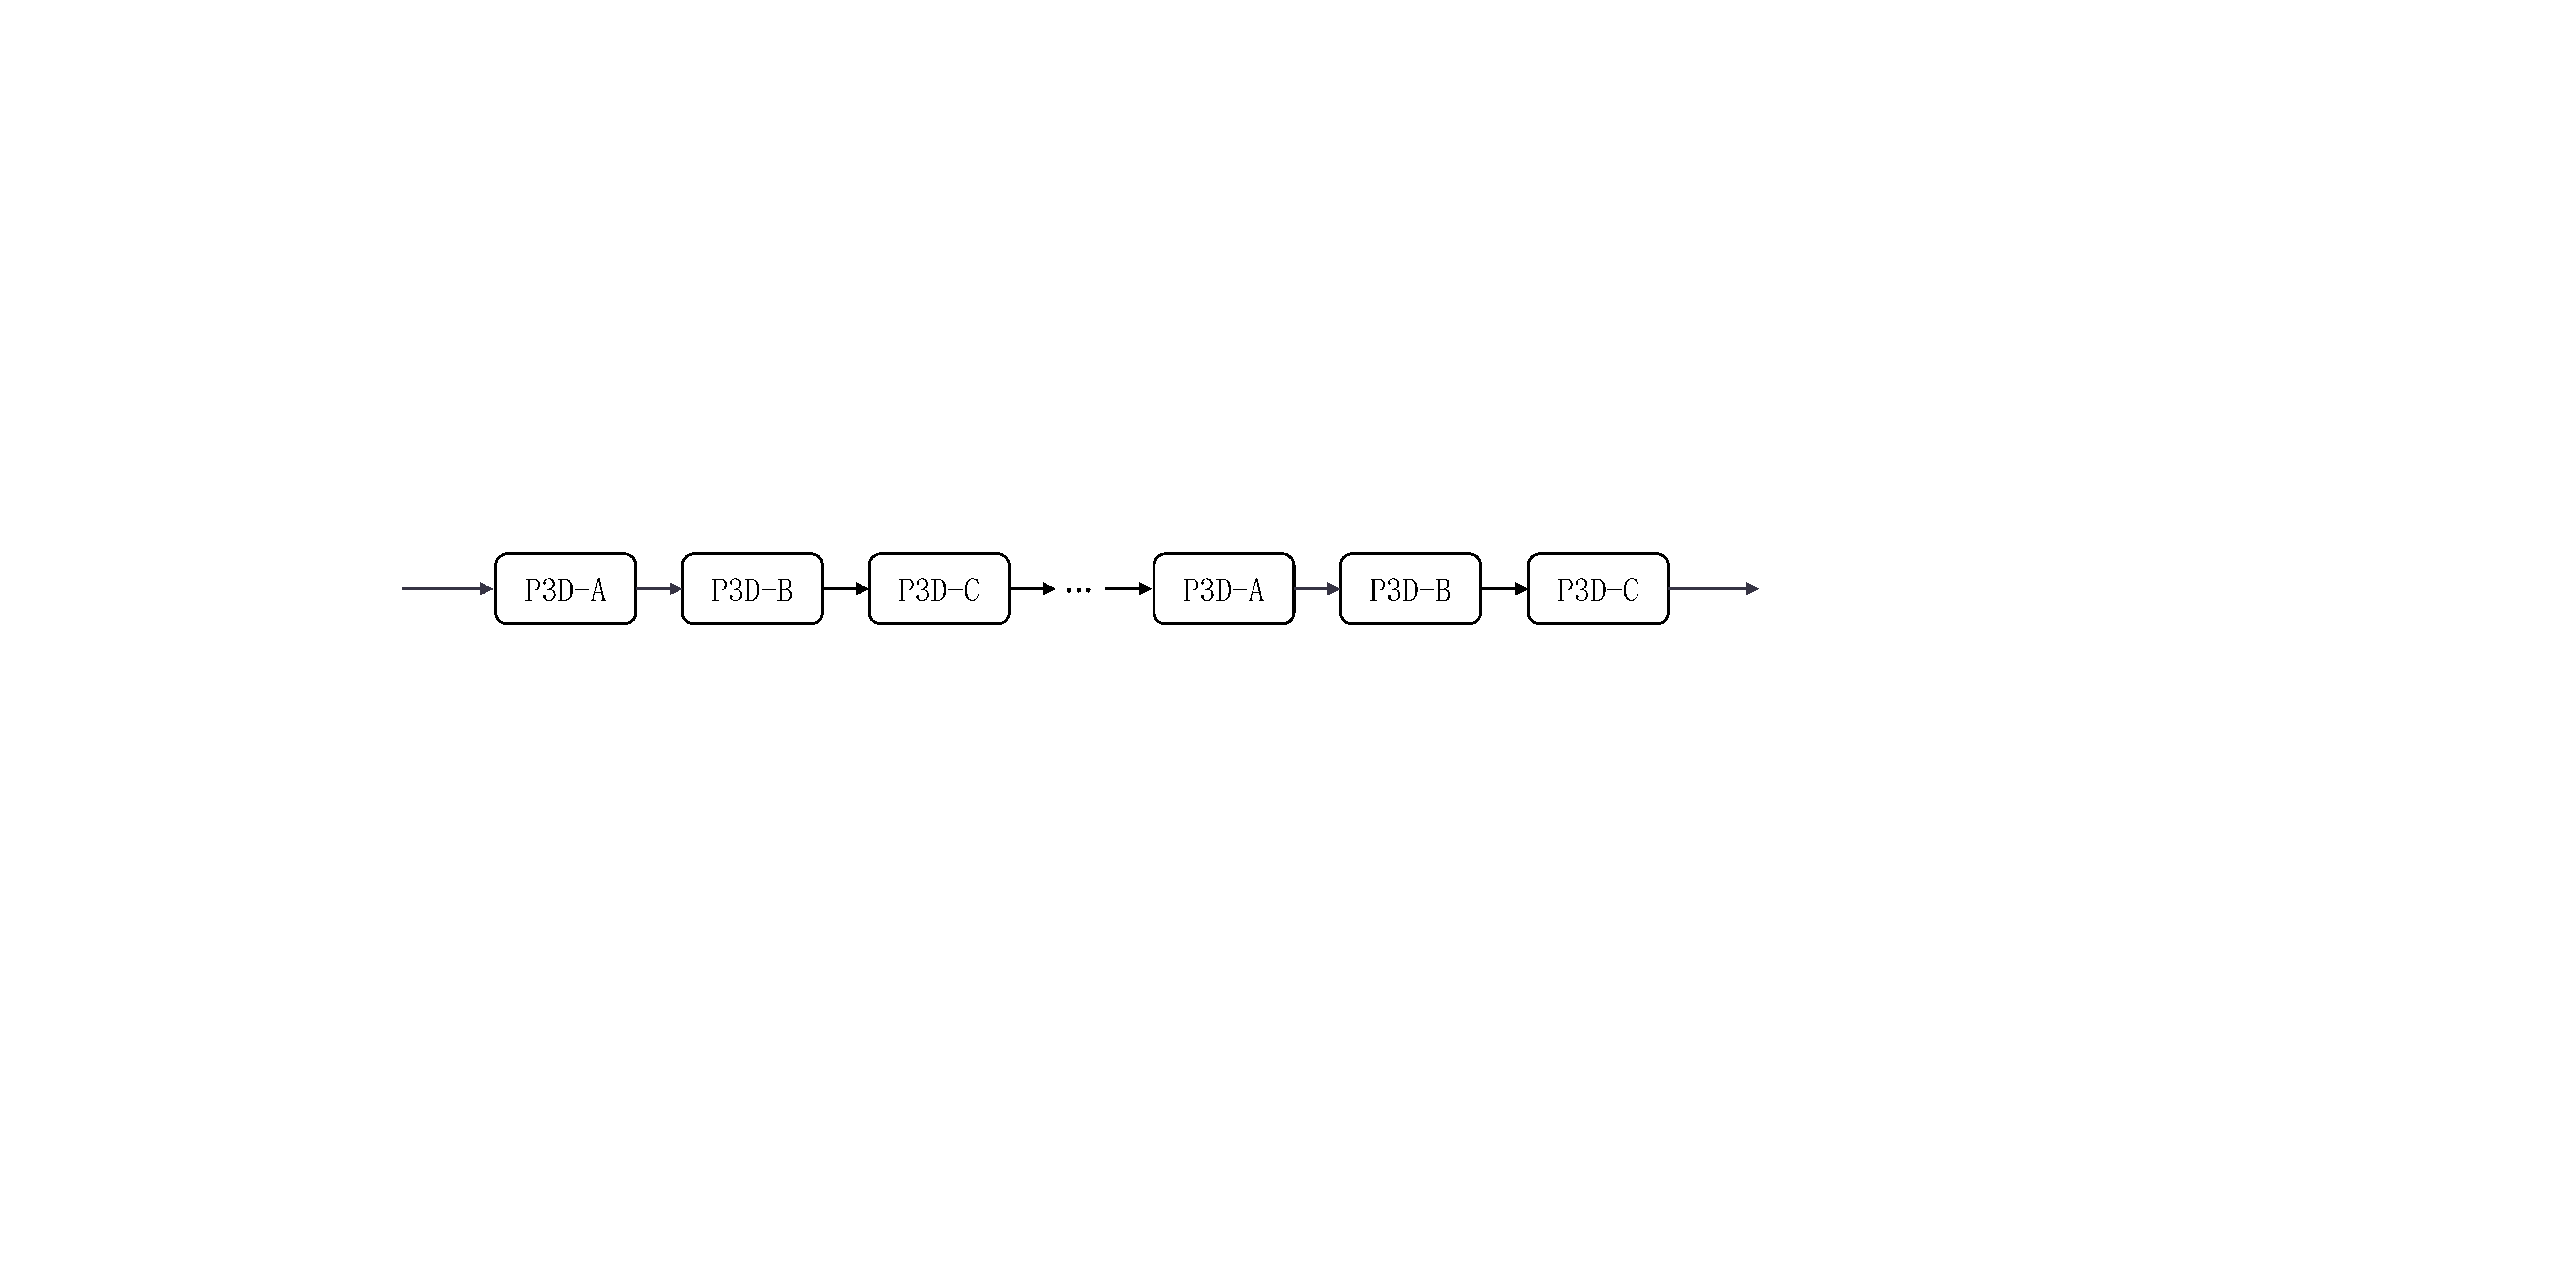
\includegraphics[width=0.80\textwidth]{P3D3}
\caption{P3D-A、P3D-B、P3D-C级联的P3D残差网络}
\label{fig24}
\end{figure}

\section{实验设置及分析}

\subsection{数据增强}

\begin{figure}[!htbp]
    \centering
    \quad
    \begin{subfigure}[b]{0.225\textwidth}
      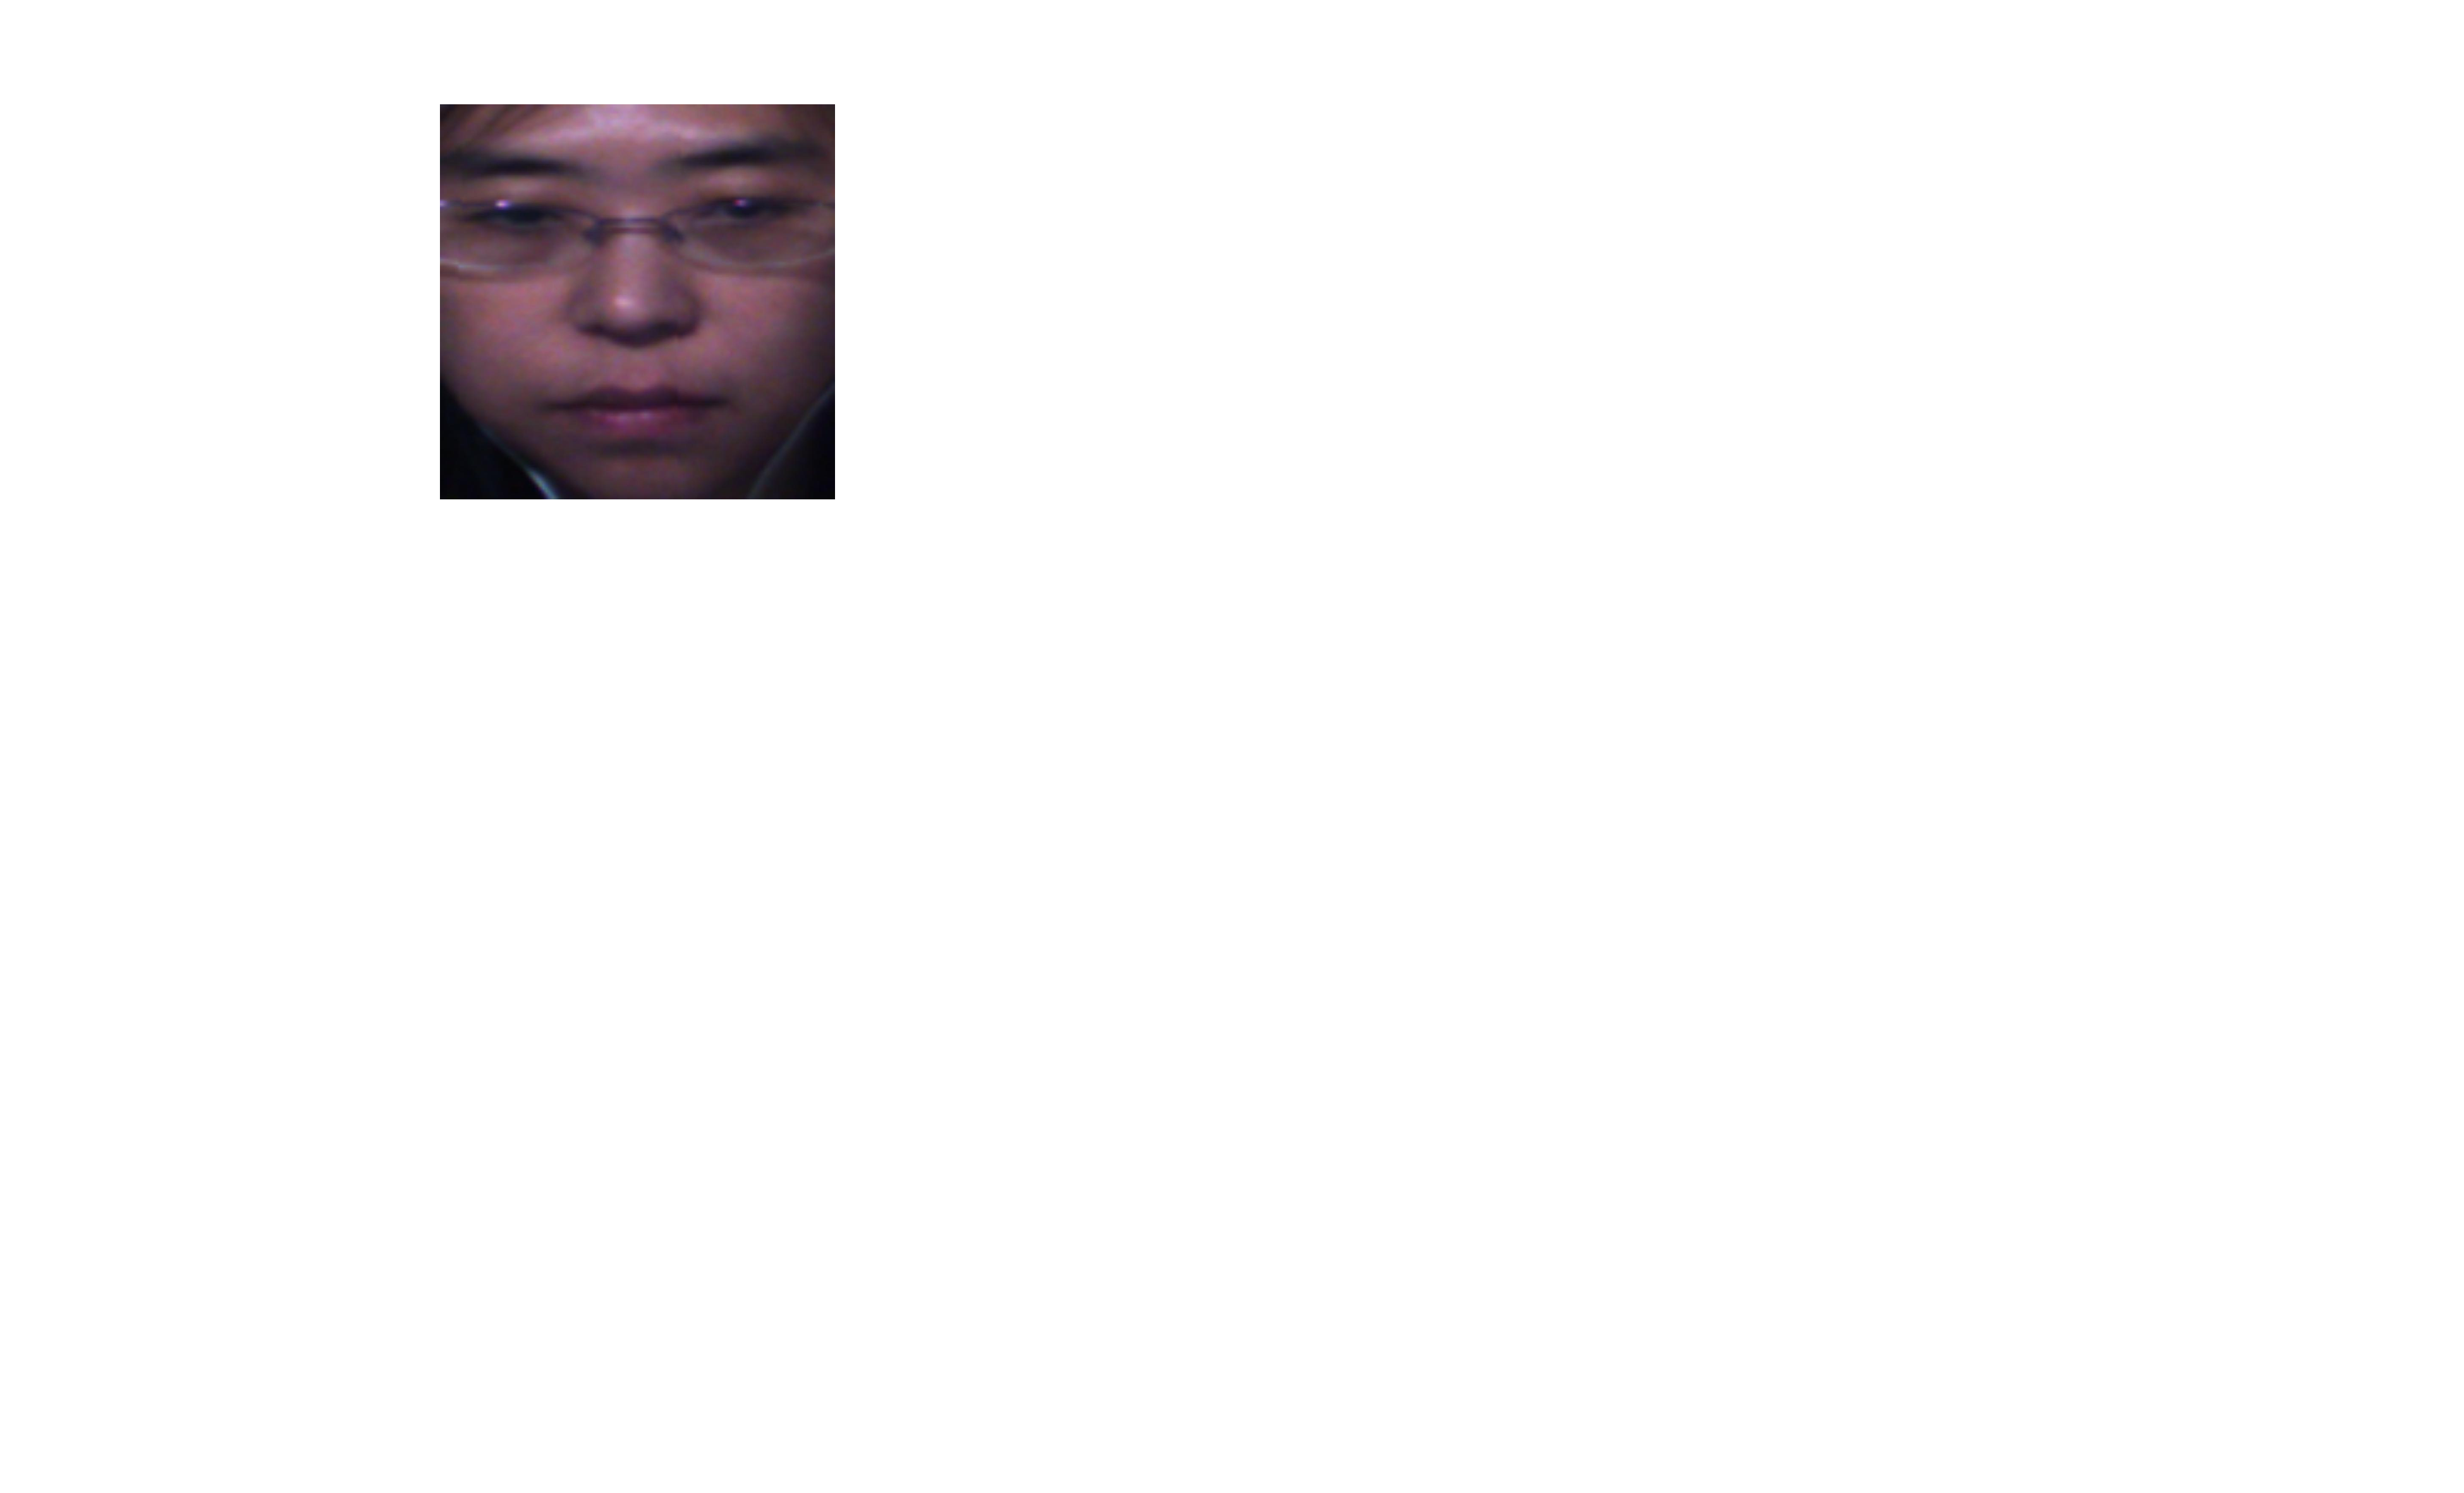
\includegraphics[width=\textwidth]{4LR0}
      \caption{}
    \end{subfigure}
    \quad
    \begin{subfigure}[b]{0.25\textwidth}
      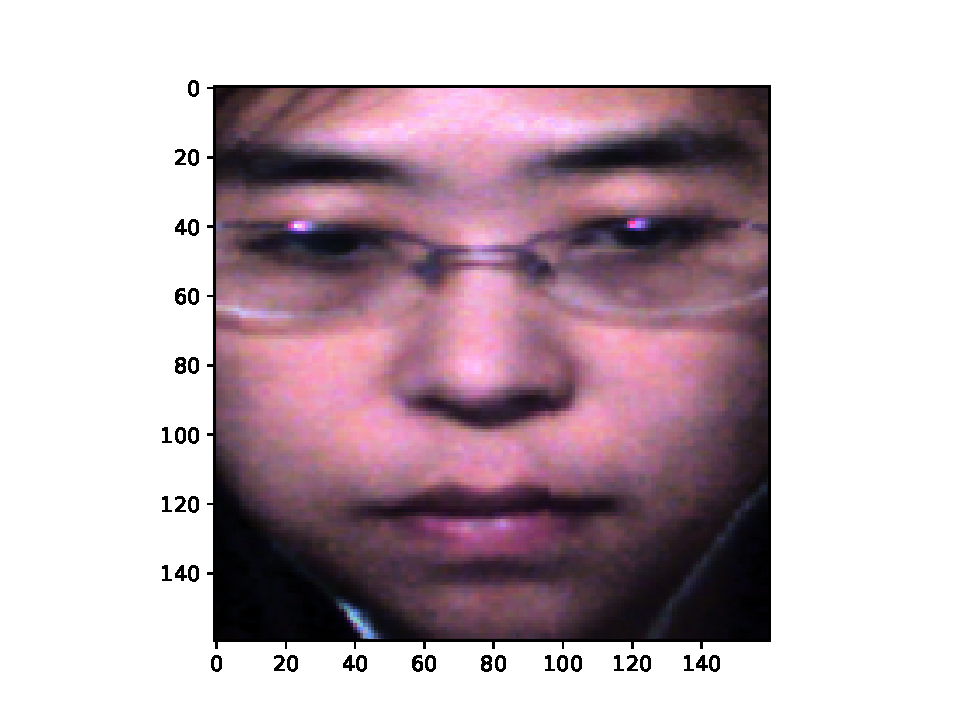
\includegraphics[width=\textwidth]{4LR2}
      \caption{}
    \end{subfigure}
    \\
    \begin{subfigure}[b]{0.25\textwidth}
      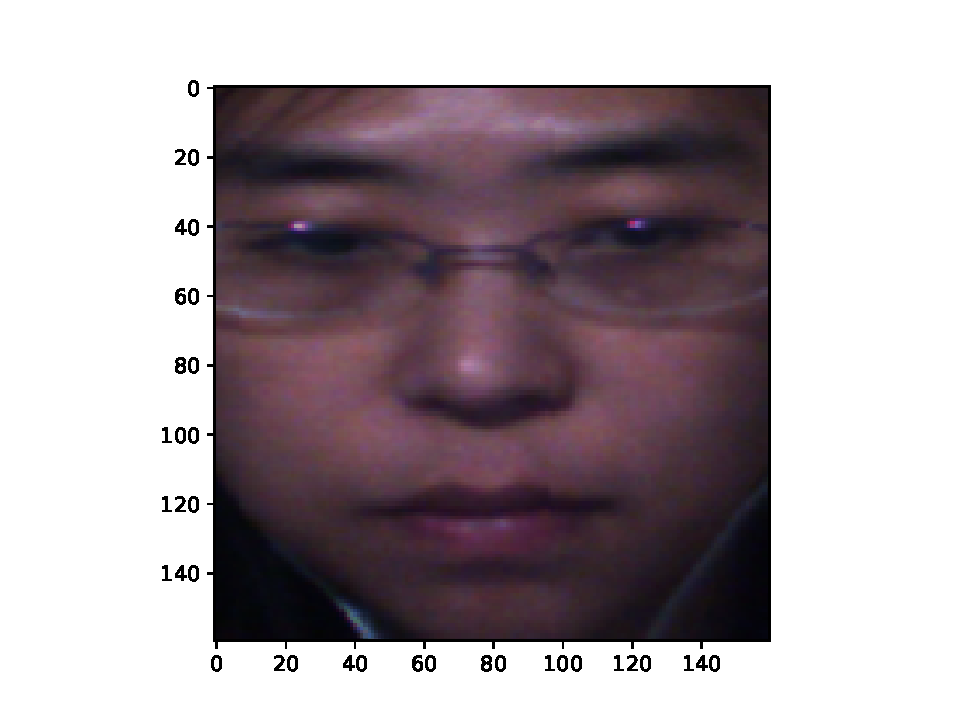
\includegraphics[width=\textwidth]{4LR3}
      \caption{}
    \end{subfigure}
    \quad
    \begin{subfigure}[b]{0.25\textwidth}
      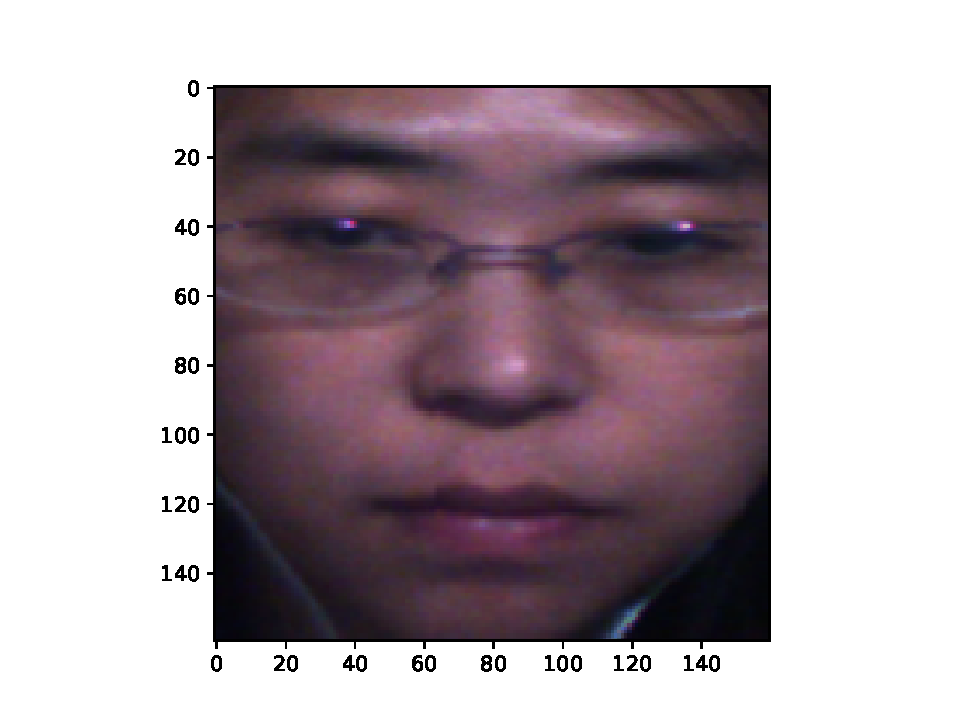
\includegraphics[width=\textwidth]{4LR4}
      \caption{}
    \end{subfigure}
    \begin{spacing}{1.0}
    \caption{直方图均衡化样例}
    \label{fig21}
    \centerline{\footnotesize \textmd{(a) 原图,(b) 直方图均衡化结果,(c) 图像亮度变化结果,(d) 水平翻转结果}}
    \end{spacing}
\end{figure}



% \begin{figure}[!htbp]
%     \centering
%     \begin{subfigure}[b]{0.225\textwidth}
%       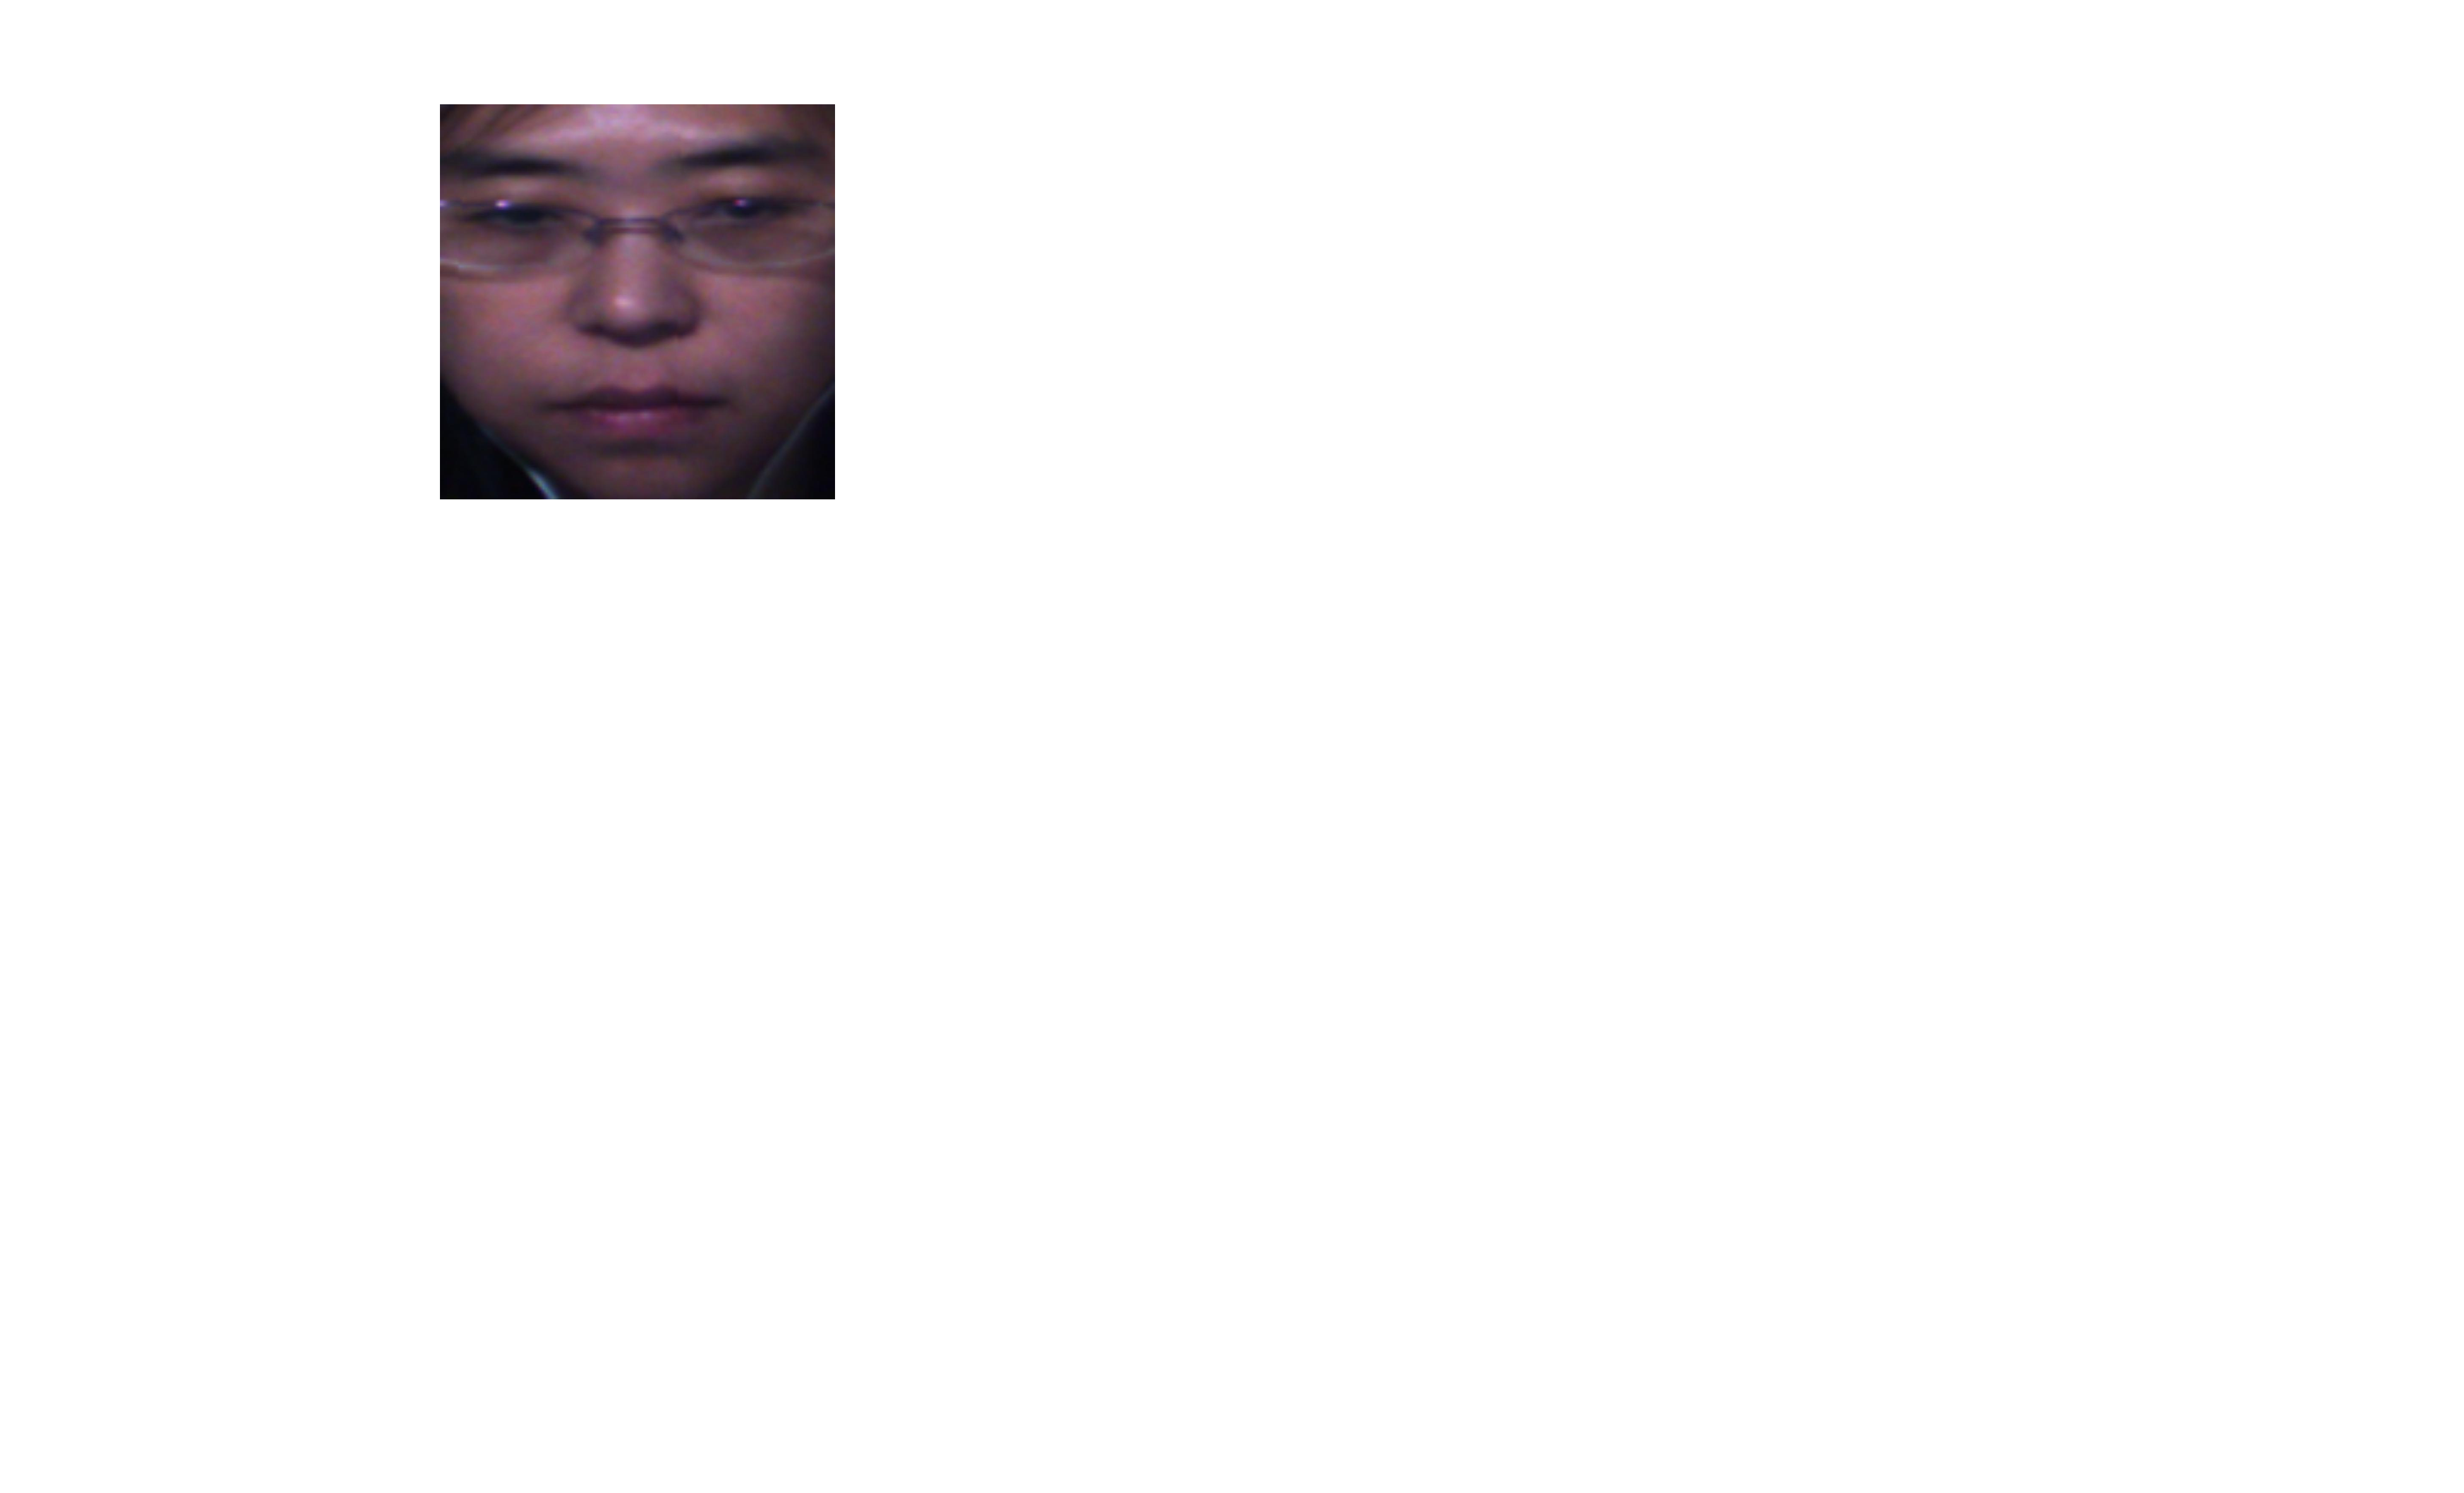
\includegraphics[width=\textwidth]{4LR0}
%       \caption{}
%     \end{subfigure}
%     \quad
%     \quad
%     \quad
%     \begin{subfigure}[b]{0.25\textwidth}
%       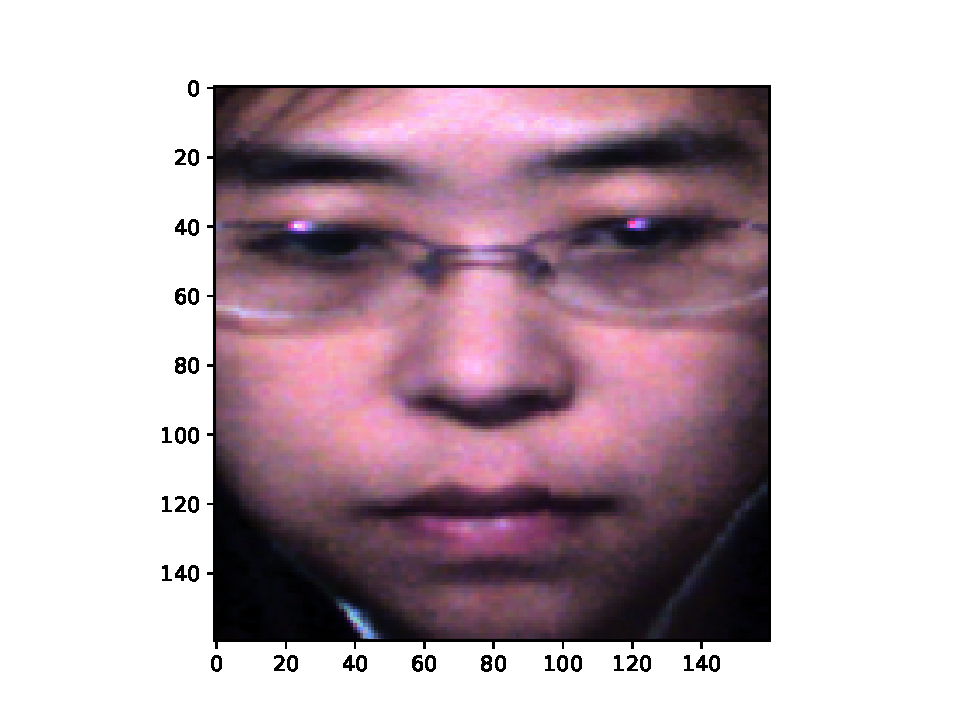
\includegraphics[width=\textwidth]{4LR2}
%       \caption{}
%     \end{subfigure}
%     \begin{spacing}{1.0}
%     \caption{直方图均衡化样例}
%     \label{fig21}
%     \centerline{\footnotesize \textmd{(a)原图,(b)直方图均衡化结果}}
%     \end{spacing}
% \end{figure}
%
% \begin{figure}[!htbp]
%     \centering
%     \begin{subfigure}[b]{0.225\textwidth}
%       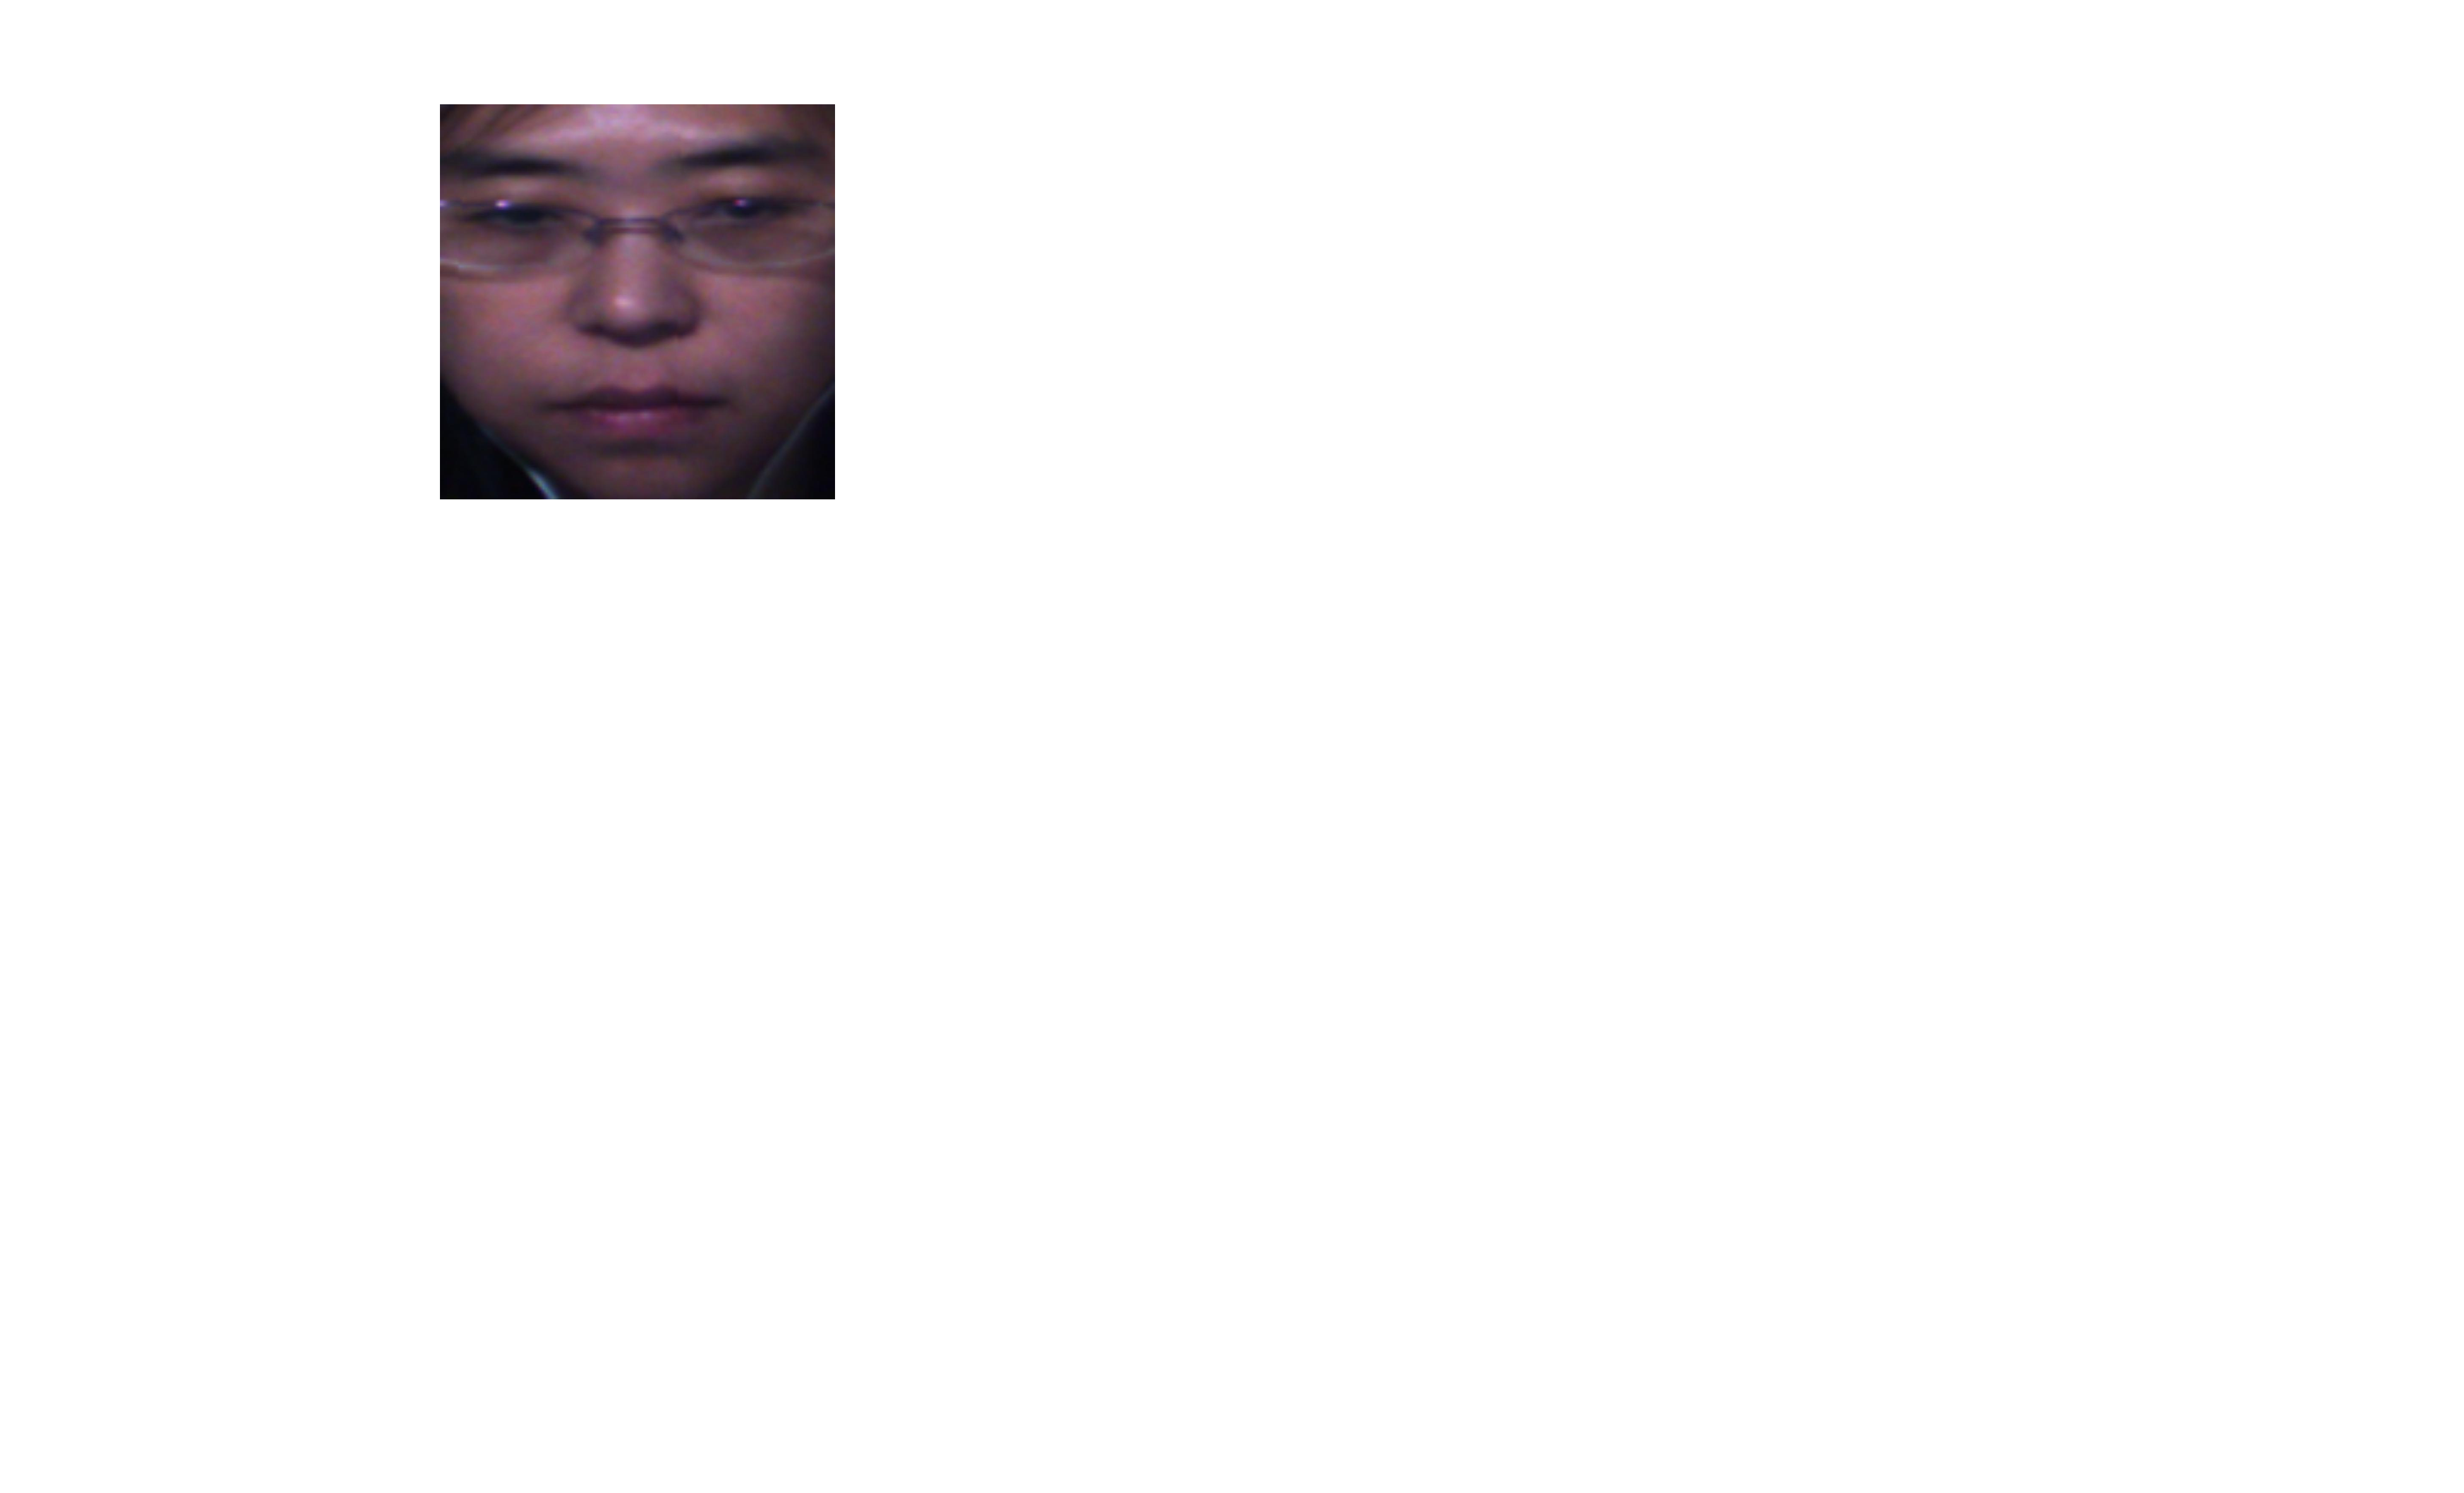
\includegraphics[width=\textwidth]{4LR0}
%       \caption{}
%     \end{subfigure}
%     \quad
%     \quad
%     \quad
%     \begin{subfigure}[b]{0.25\textwidth}
%       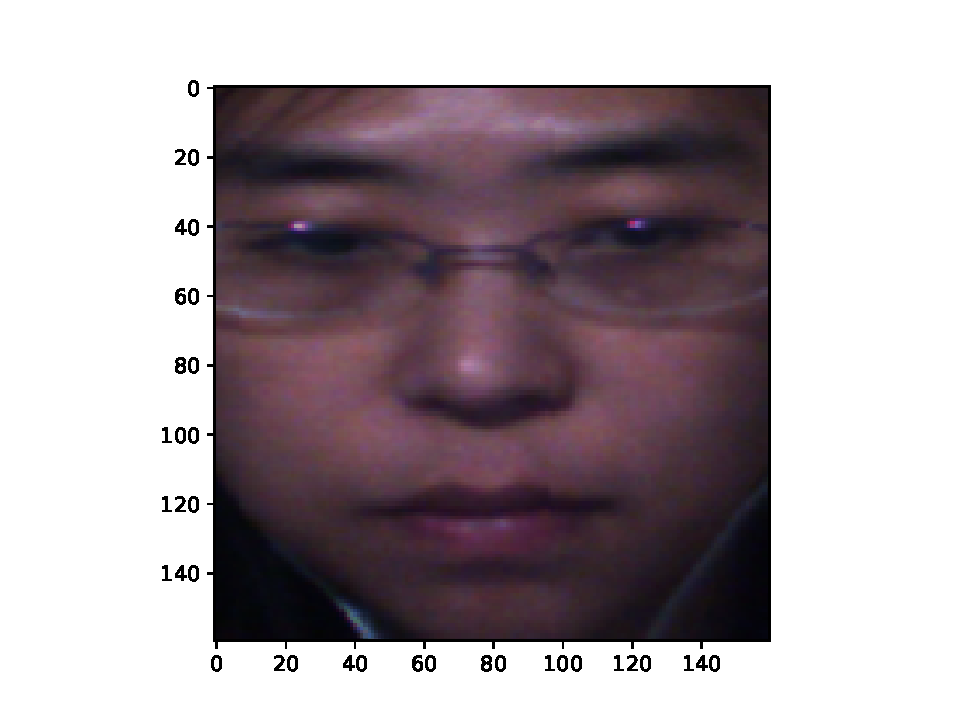
\includegraphics[width=\textwidth]{4LR3}
%       \caption{}
%     \end{subfigure}
%     \begin{spacing}{1.0}
%     \caption{图像亮度变化样例}
%     \label{fig21}
%     \centerline{\footnotesize \textmd{(a) 原图,(b) 图像亮度变化结果}}
%     \end{spacing}
% \end{figure}
%
% \begin{figure}[!htbp]
%     \centering
%     \begin{subfigure}[b]{0.225\textwidth}
%       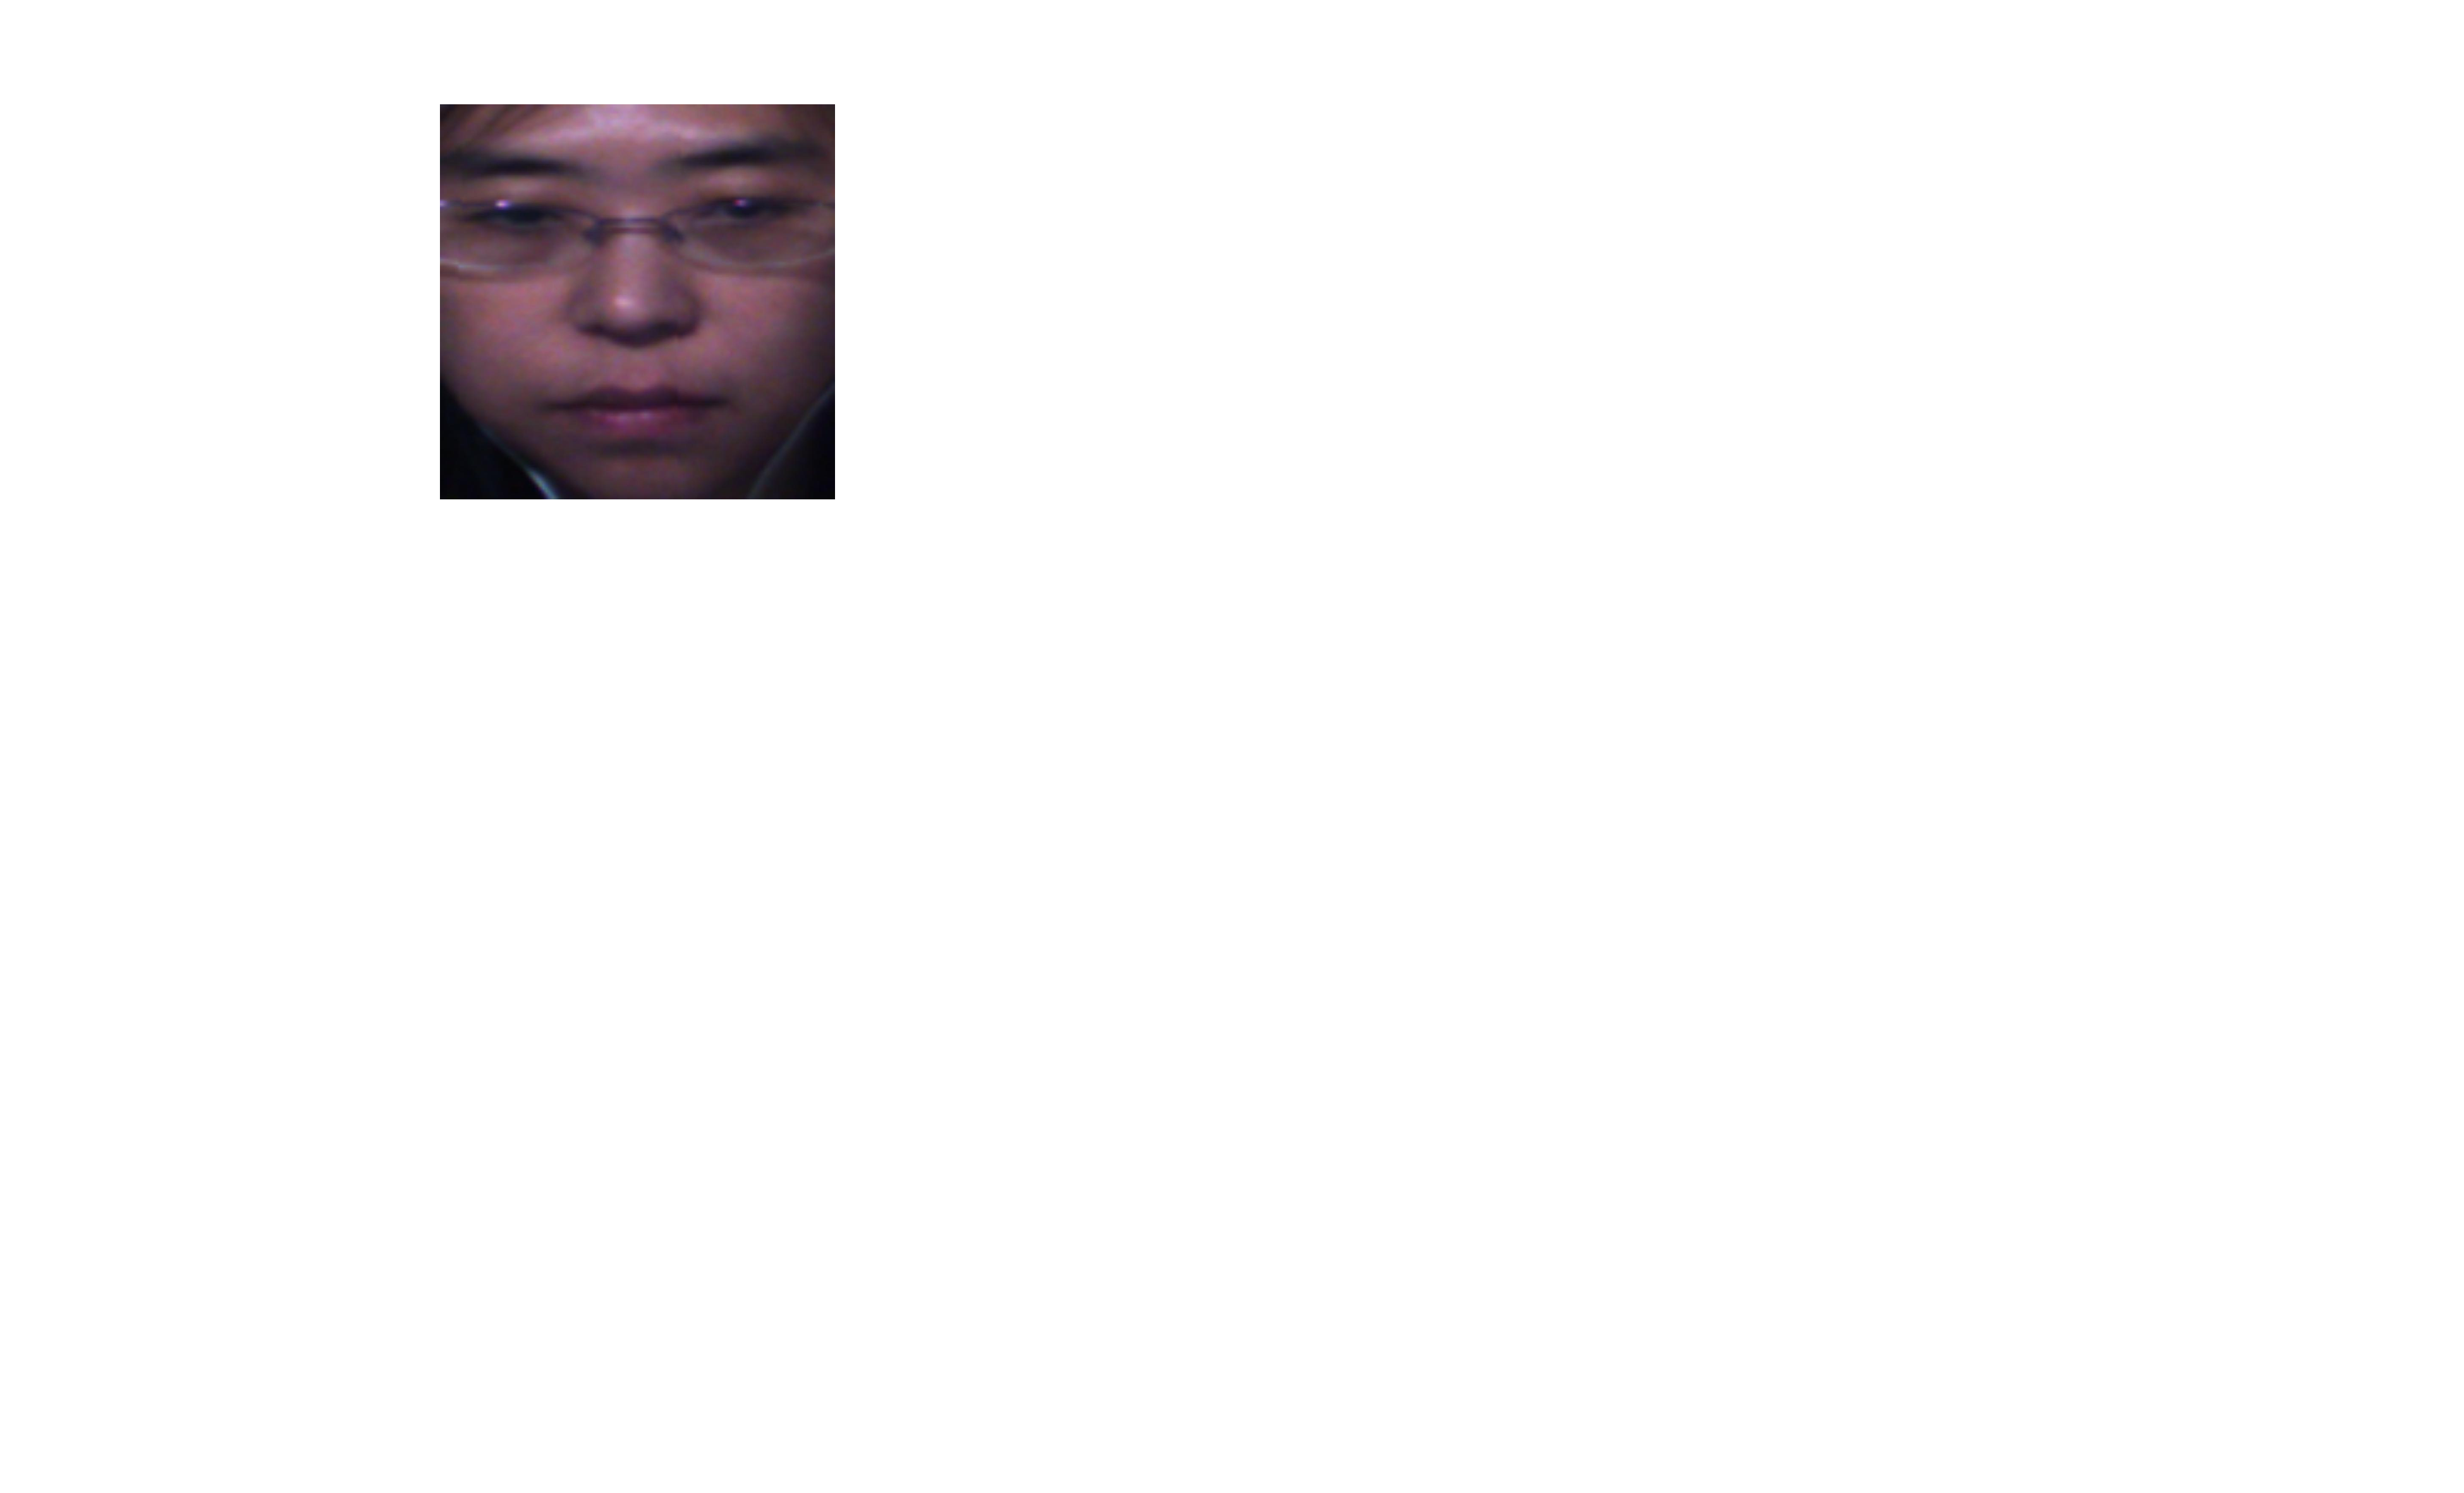
\includegraphics[width=\textwidth]{4LR0}
%       \caption{}
%     \end{subfigure}
%     \quad
%     \quad
%     \quad
%     \begin{subfigure}[b]{0.25\textwidth}
%       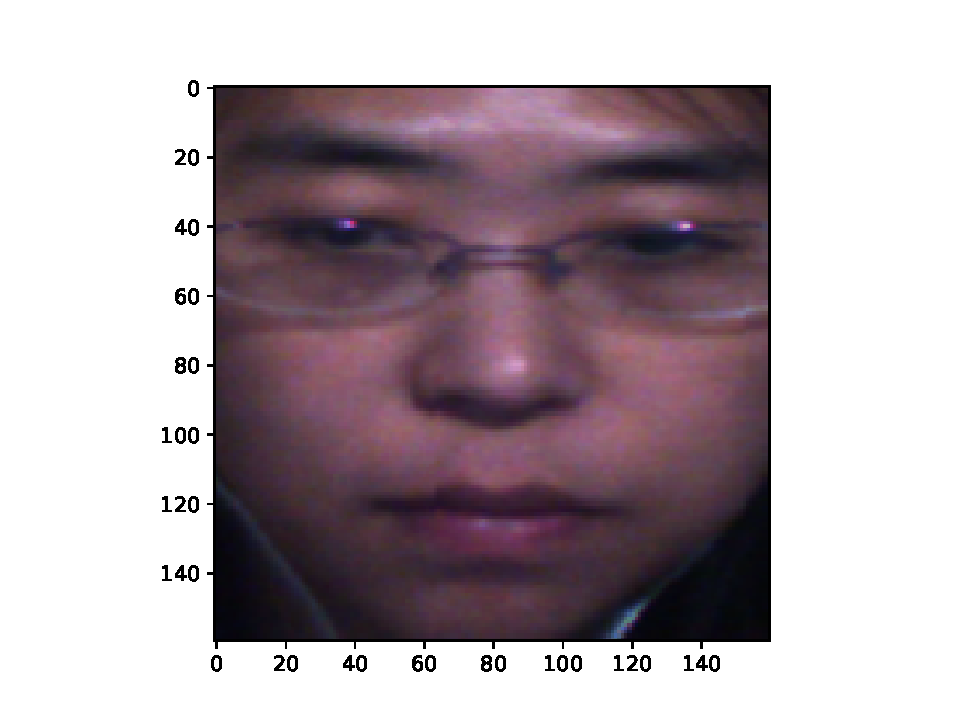
\includegraphics[width=\textwidth]{4LR4}
%       \caption{}
%     \end{subfigure}
%     \begin{spacing}{1.0}
%     \caption{水平翻转样例}
%     \label{fig21}
%     \centerline{\footnotesize \textmd{(a) 原图,(b) 水平翻转结果}}
%     \end{spacing}
% \end{figure}

\subsection{特征提取及识别}

\section{本章小结}
